\section{Dependent Random Variables}

Let's put our die and coin away to step outside.
To look at dependent random variables, we will consider a hypothetical weather scenario.
We will consider two aspects of the weather: precipitation and light.
In our hypothetical scenario, precipitation conditions may either be dry or wet.
We will model the situation with a random variable $\bm{P}$ that can take on the value ``dry'' or ``wet.''
The probability that conditions are dry is 0.9 and the probability that conditions are wet is 0.1.
\begin{center}
  \begin{tabular}{c c}
  \makecell{
    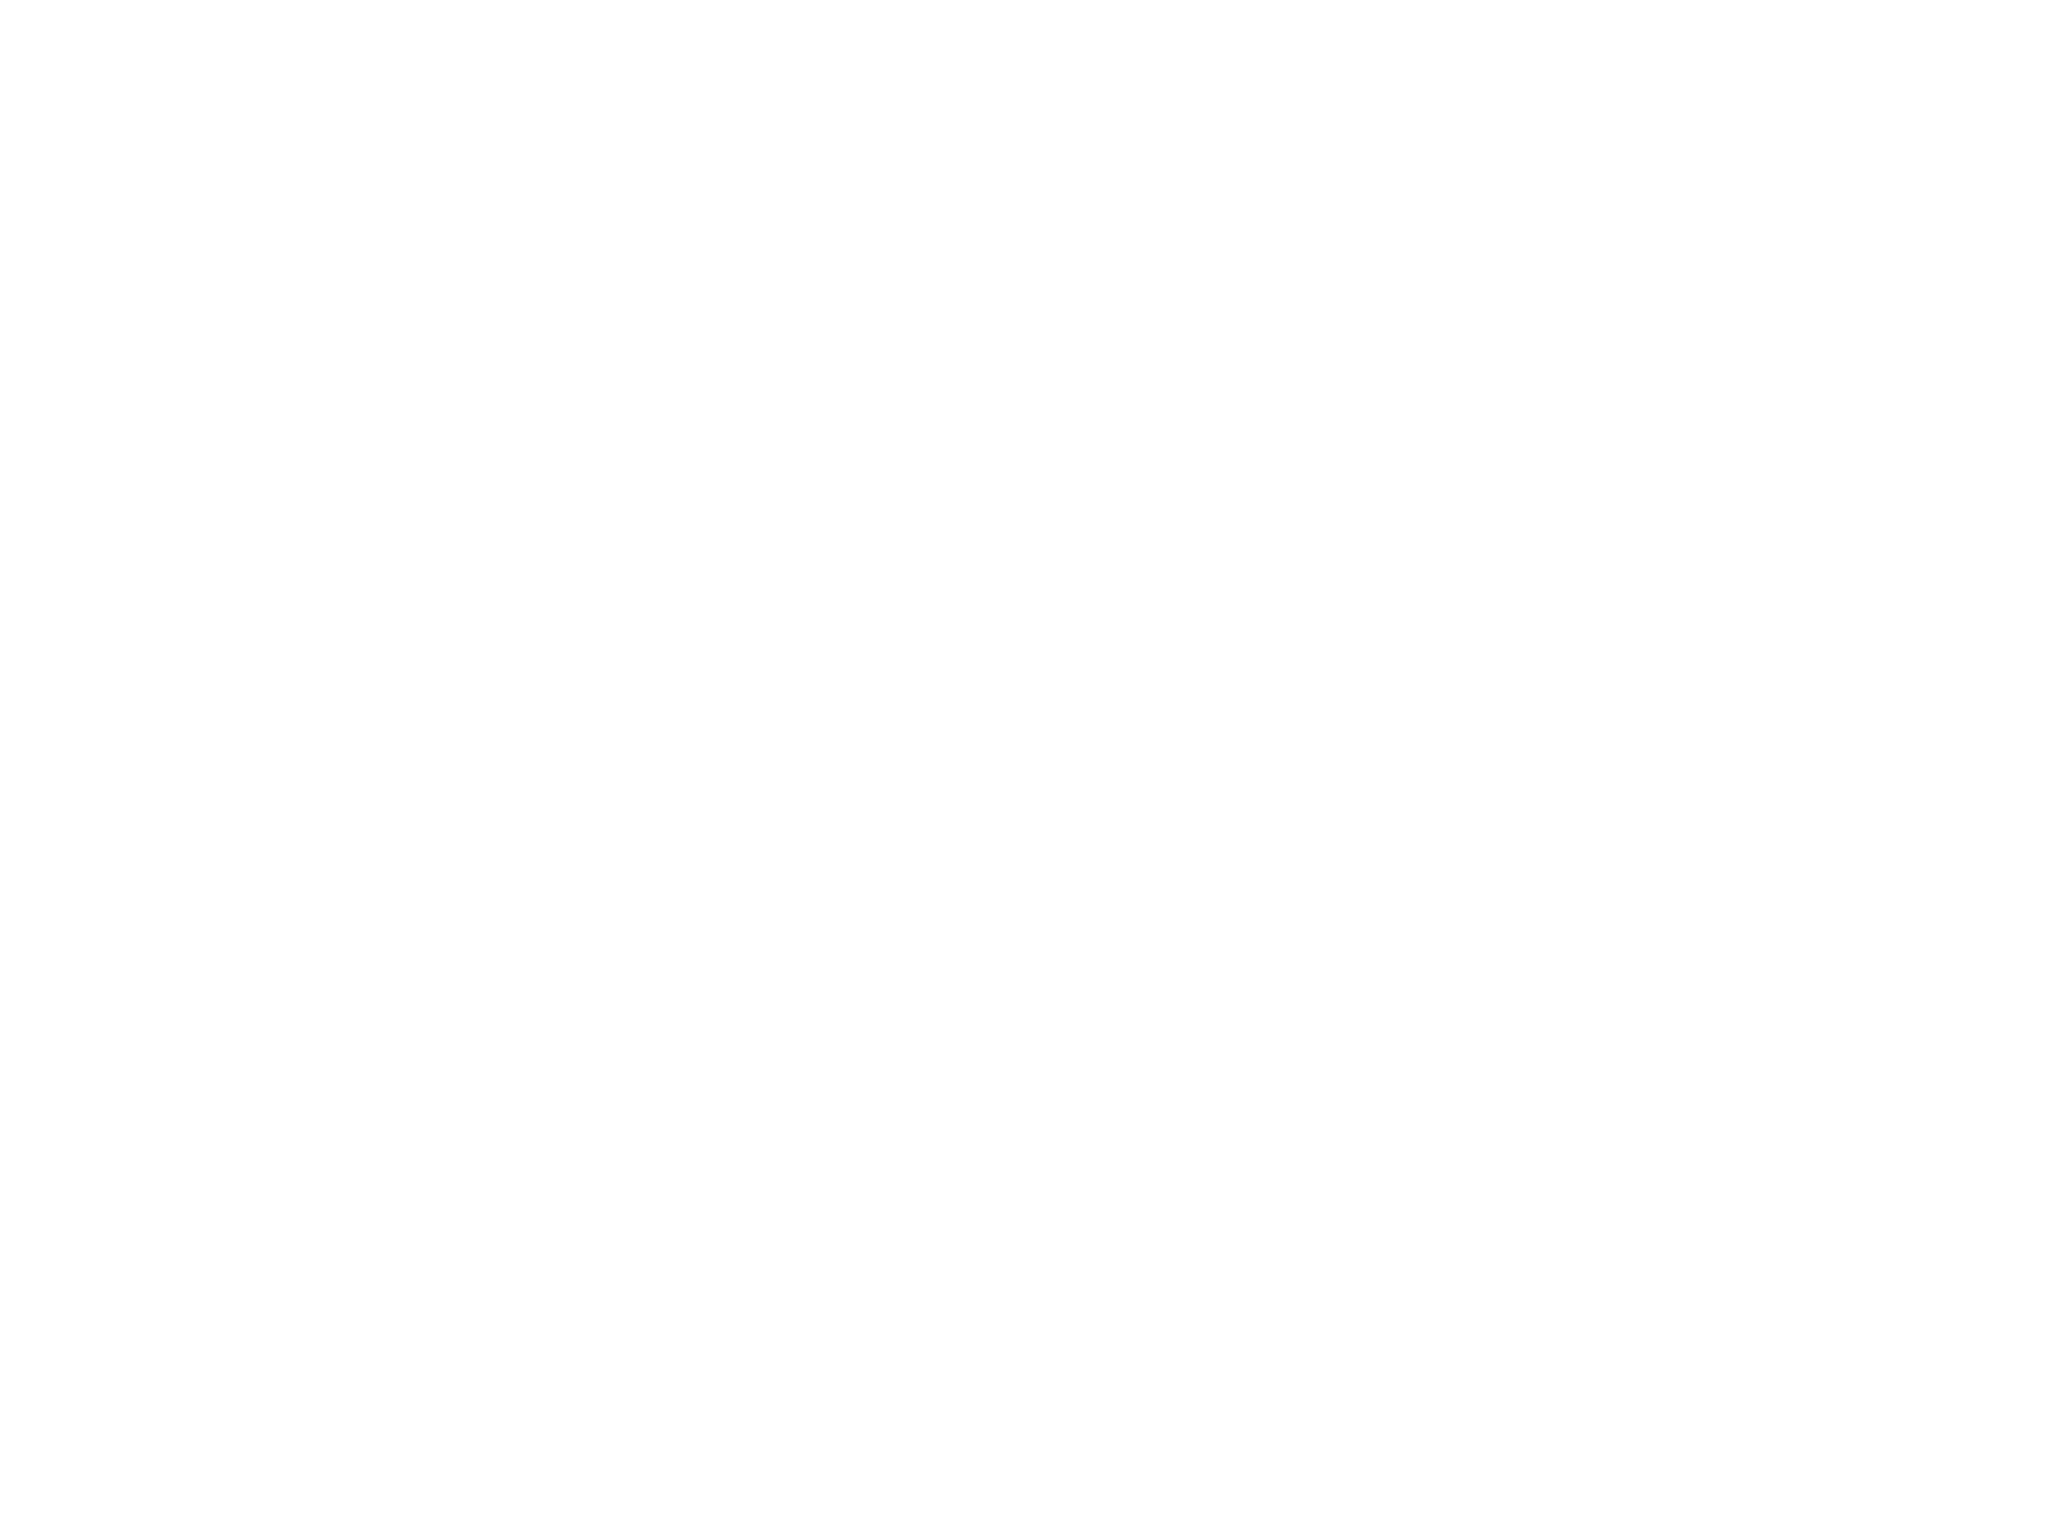
\includegraphics[width=0.5\textwidth]{img/dry} \\
    $p_{\bm{P} = \text{dry}} = 0.9$
    }
  &
  \makecell{
    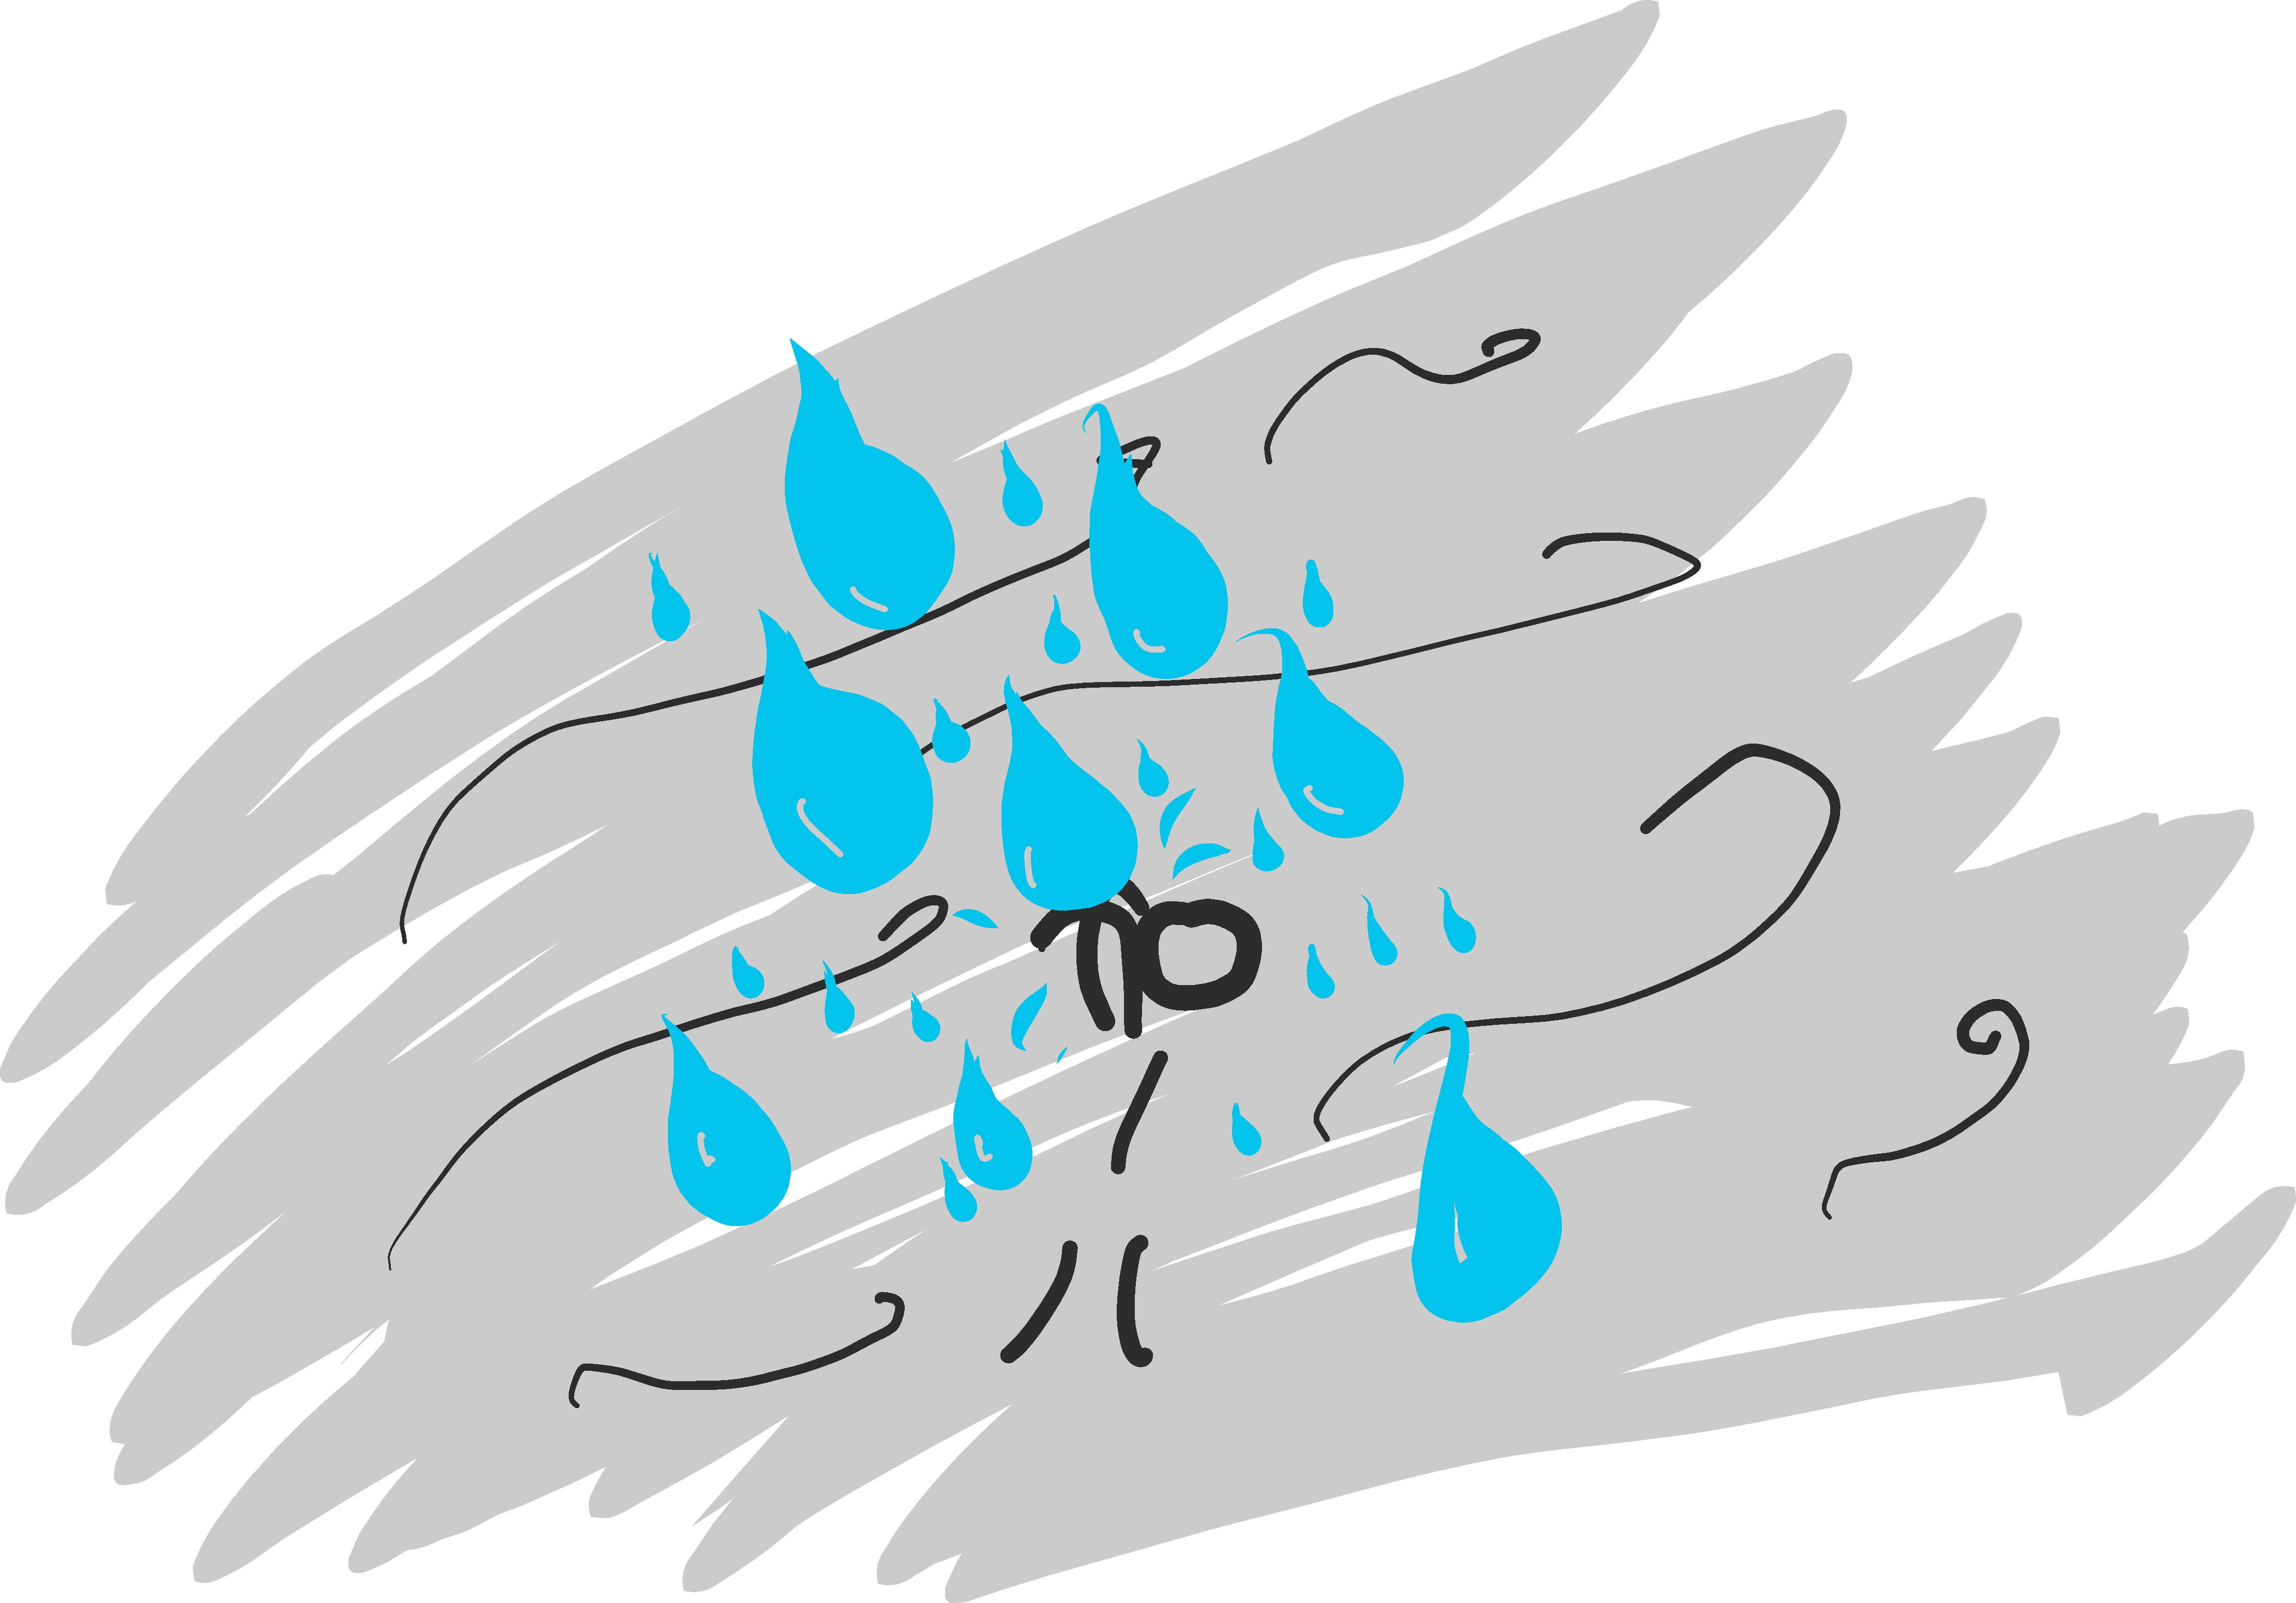
\includegraphics[width=0.3\textwidth]{img/rain} \\
    $p_{\bm{P} = \text{wet}} = 0.1$
    }
  \end{tabular}
\end{center}
Similarly, we model light conditions with a random variable $\bm{L}$ that can take on the value ``sunny'' or ``overcast.''
Sunny means that clouds are not currently occluding the sun (but may be present elsewhere in the sky).
Overcast means that the sun is currently occluded by cloud cover.
The probability that conditions are sunny is 0.5 and the probability that conditions are wet is 0.5.
\begin{center}
  \begin{tabular}{c c}
  \makecell{
    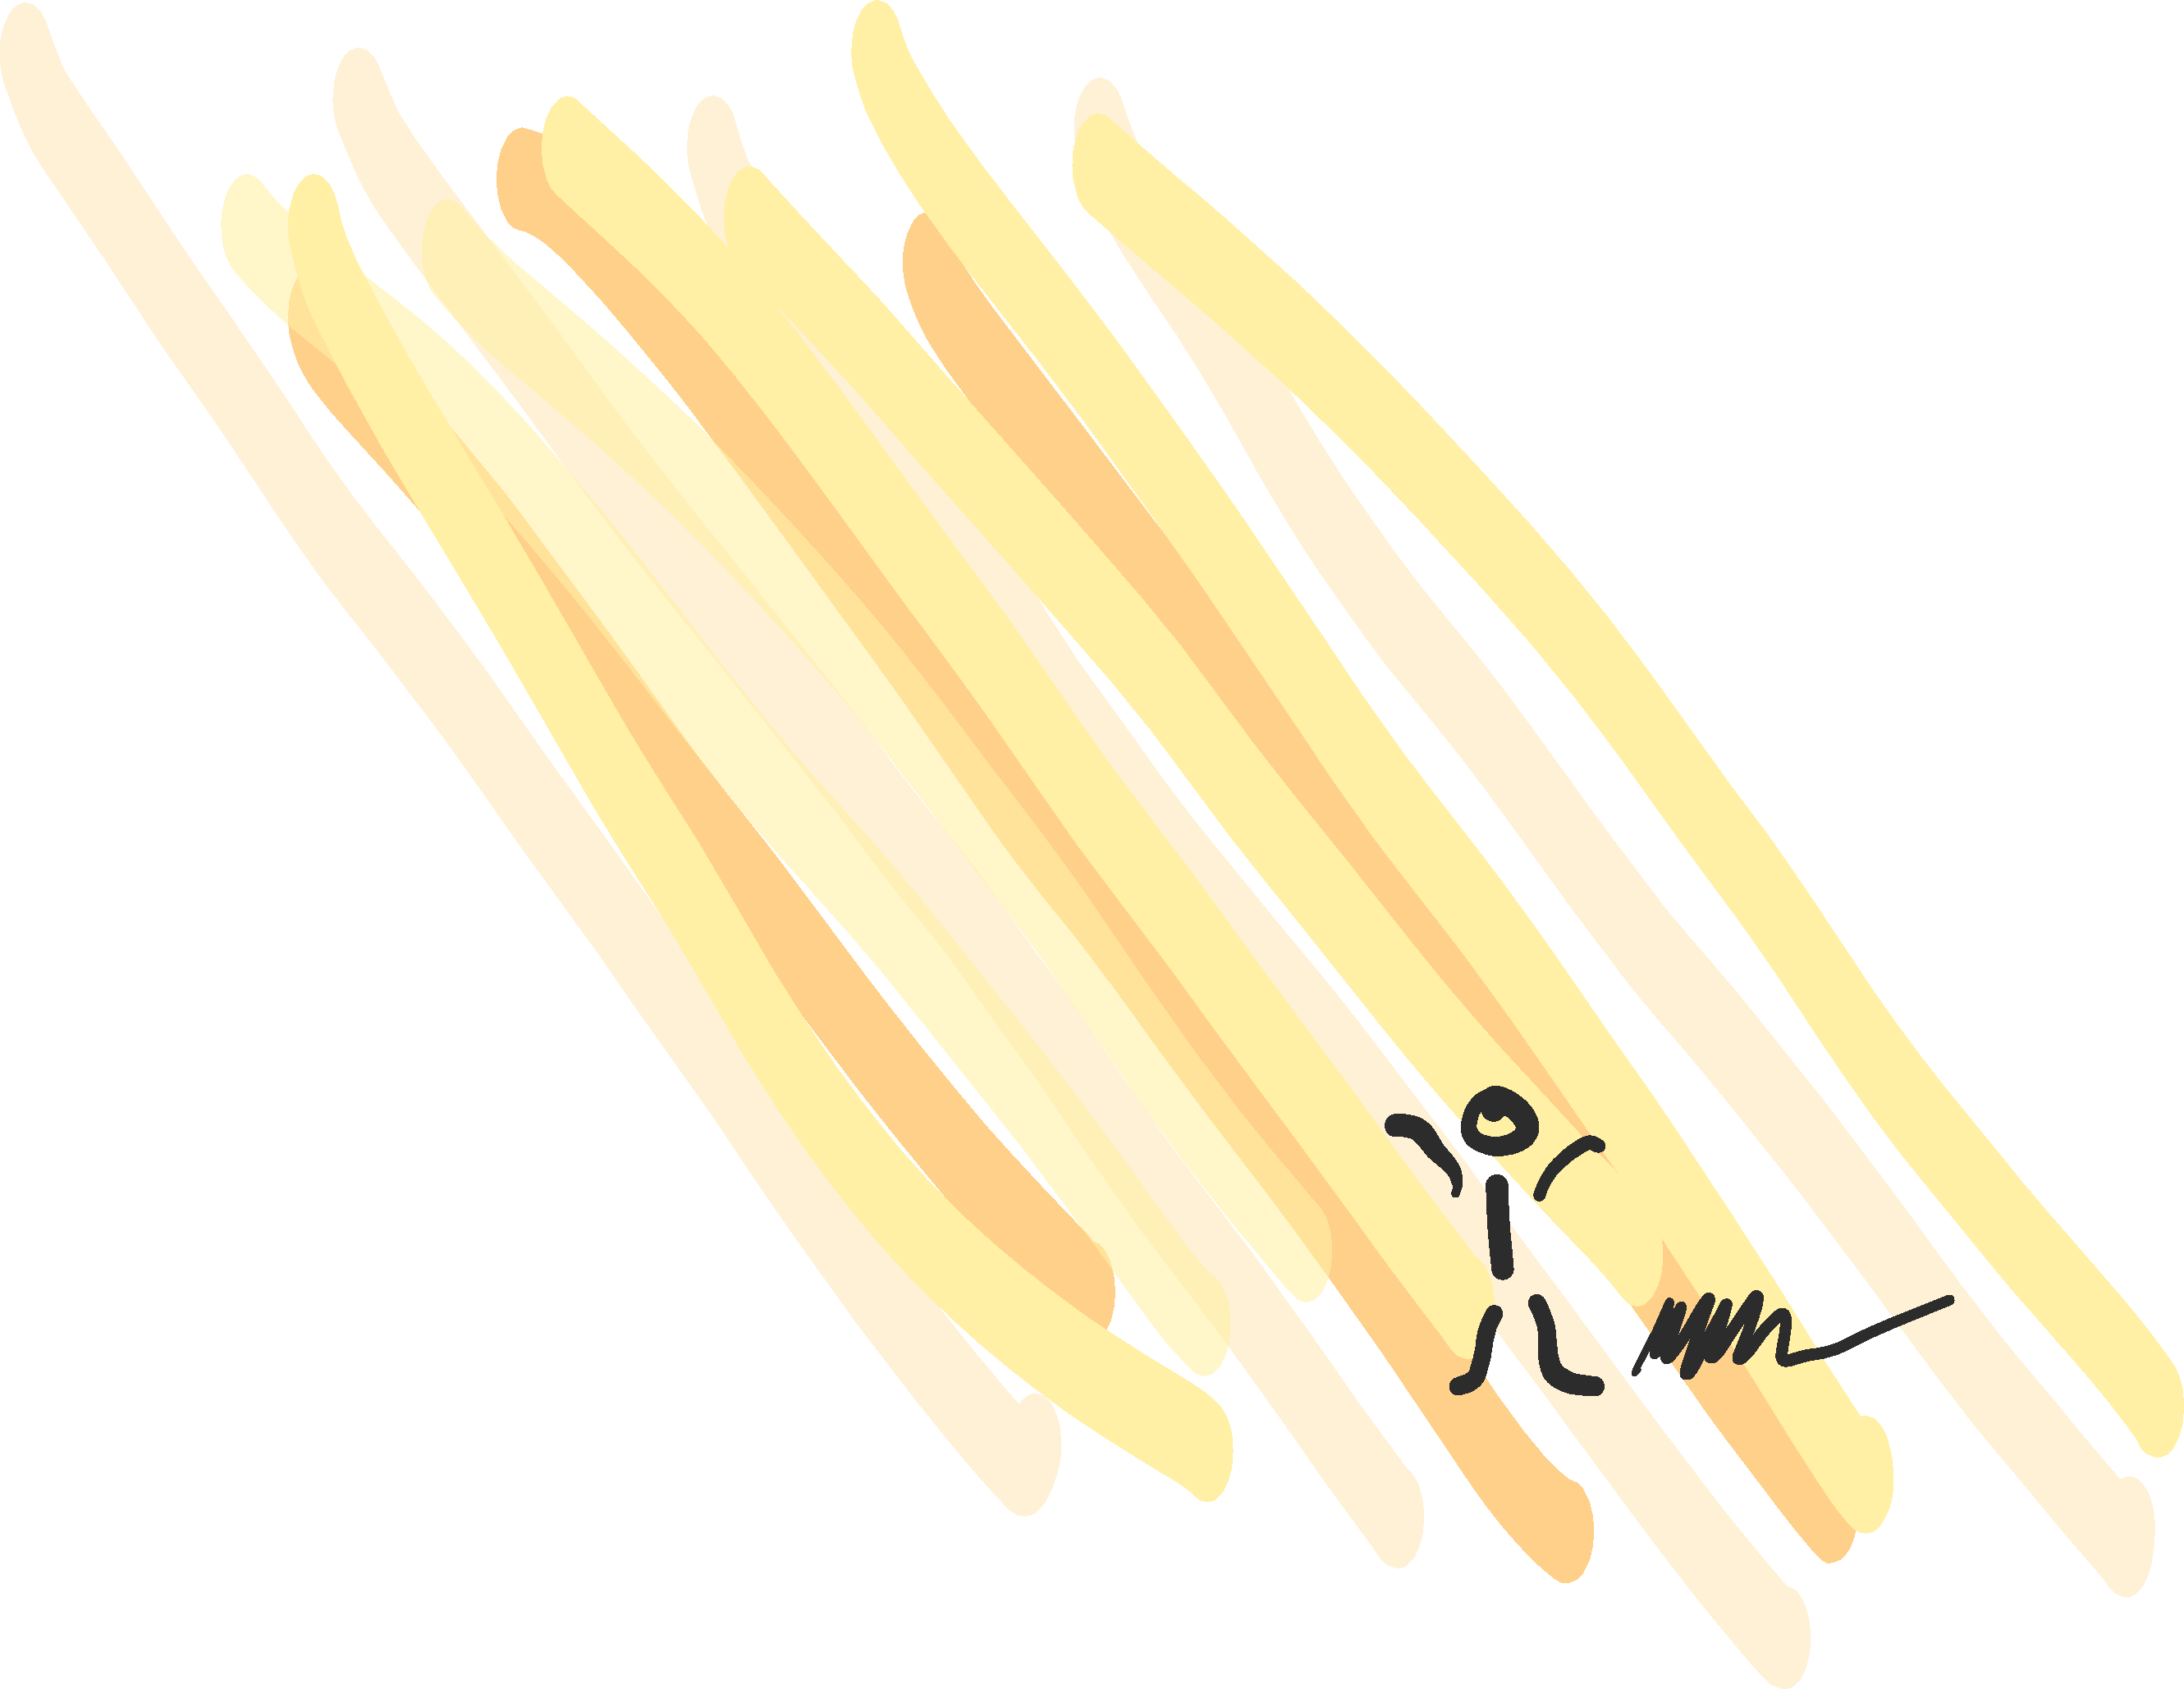
\includegraphics[width=0.3\textwidth]{img/sun} \\
    $p_{\bm{P} = \text{dry}} = 0.5$
    }
  &
  \makecell{
    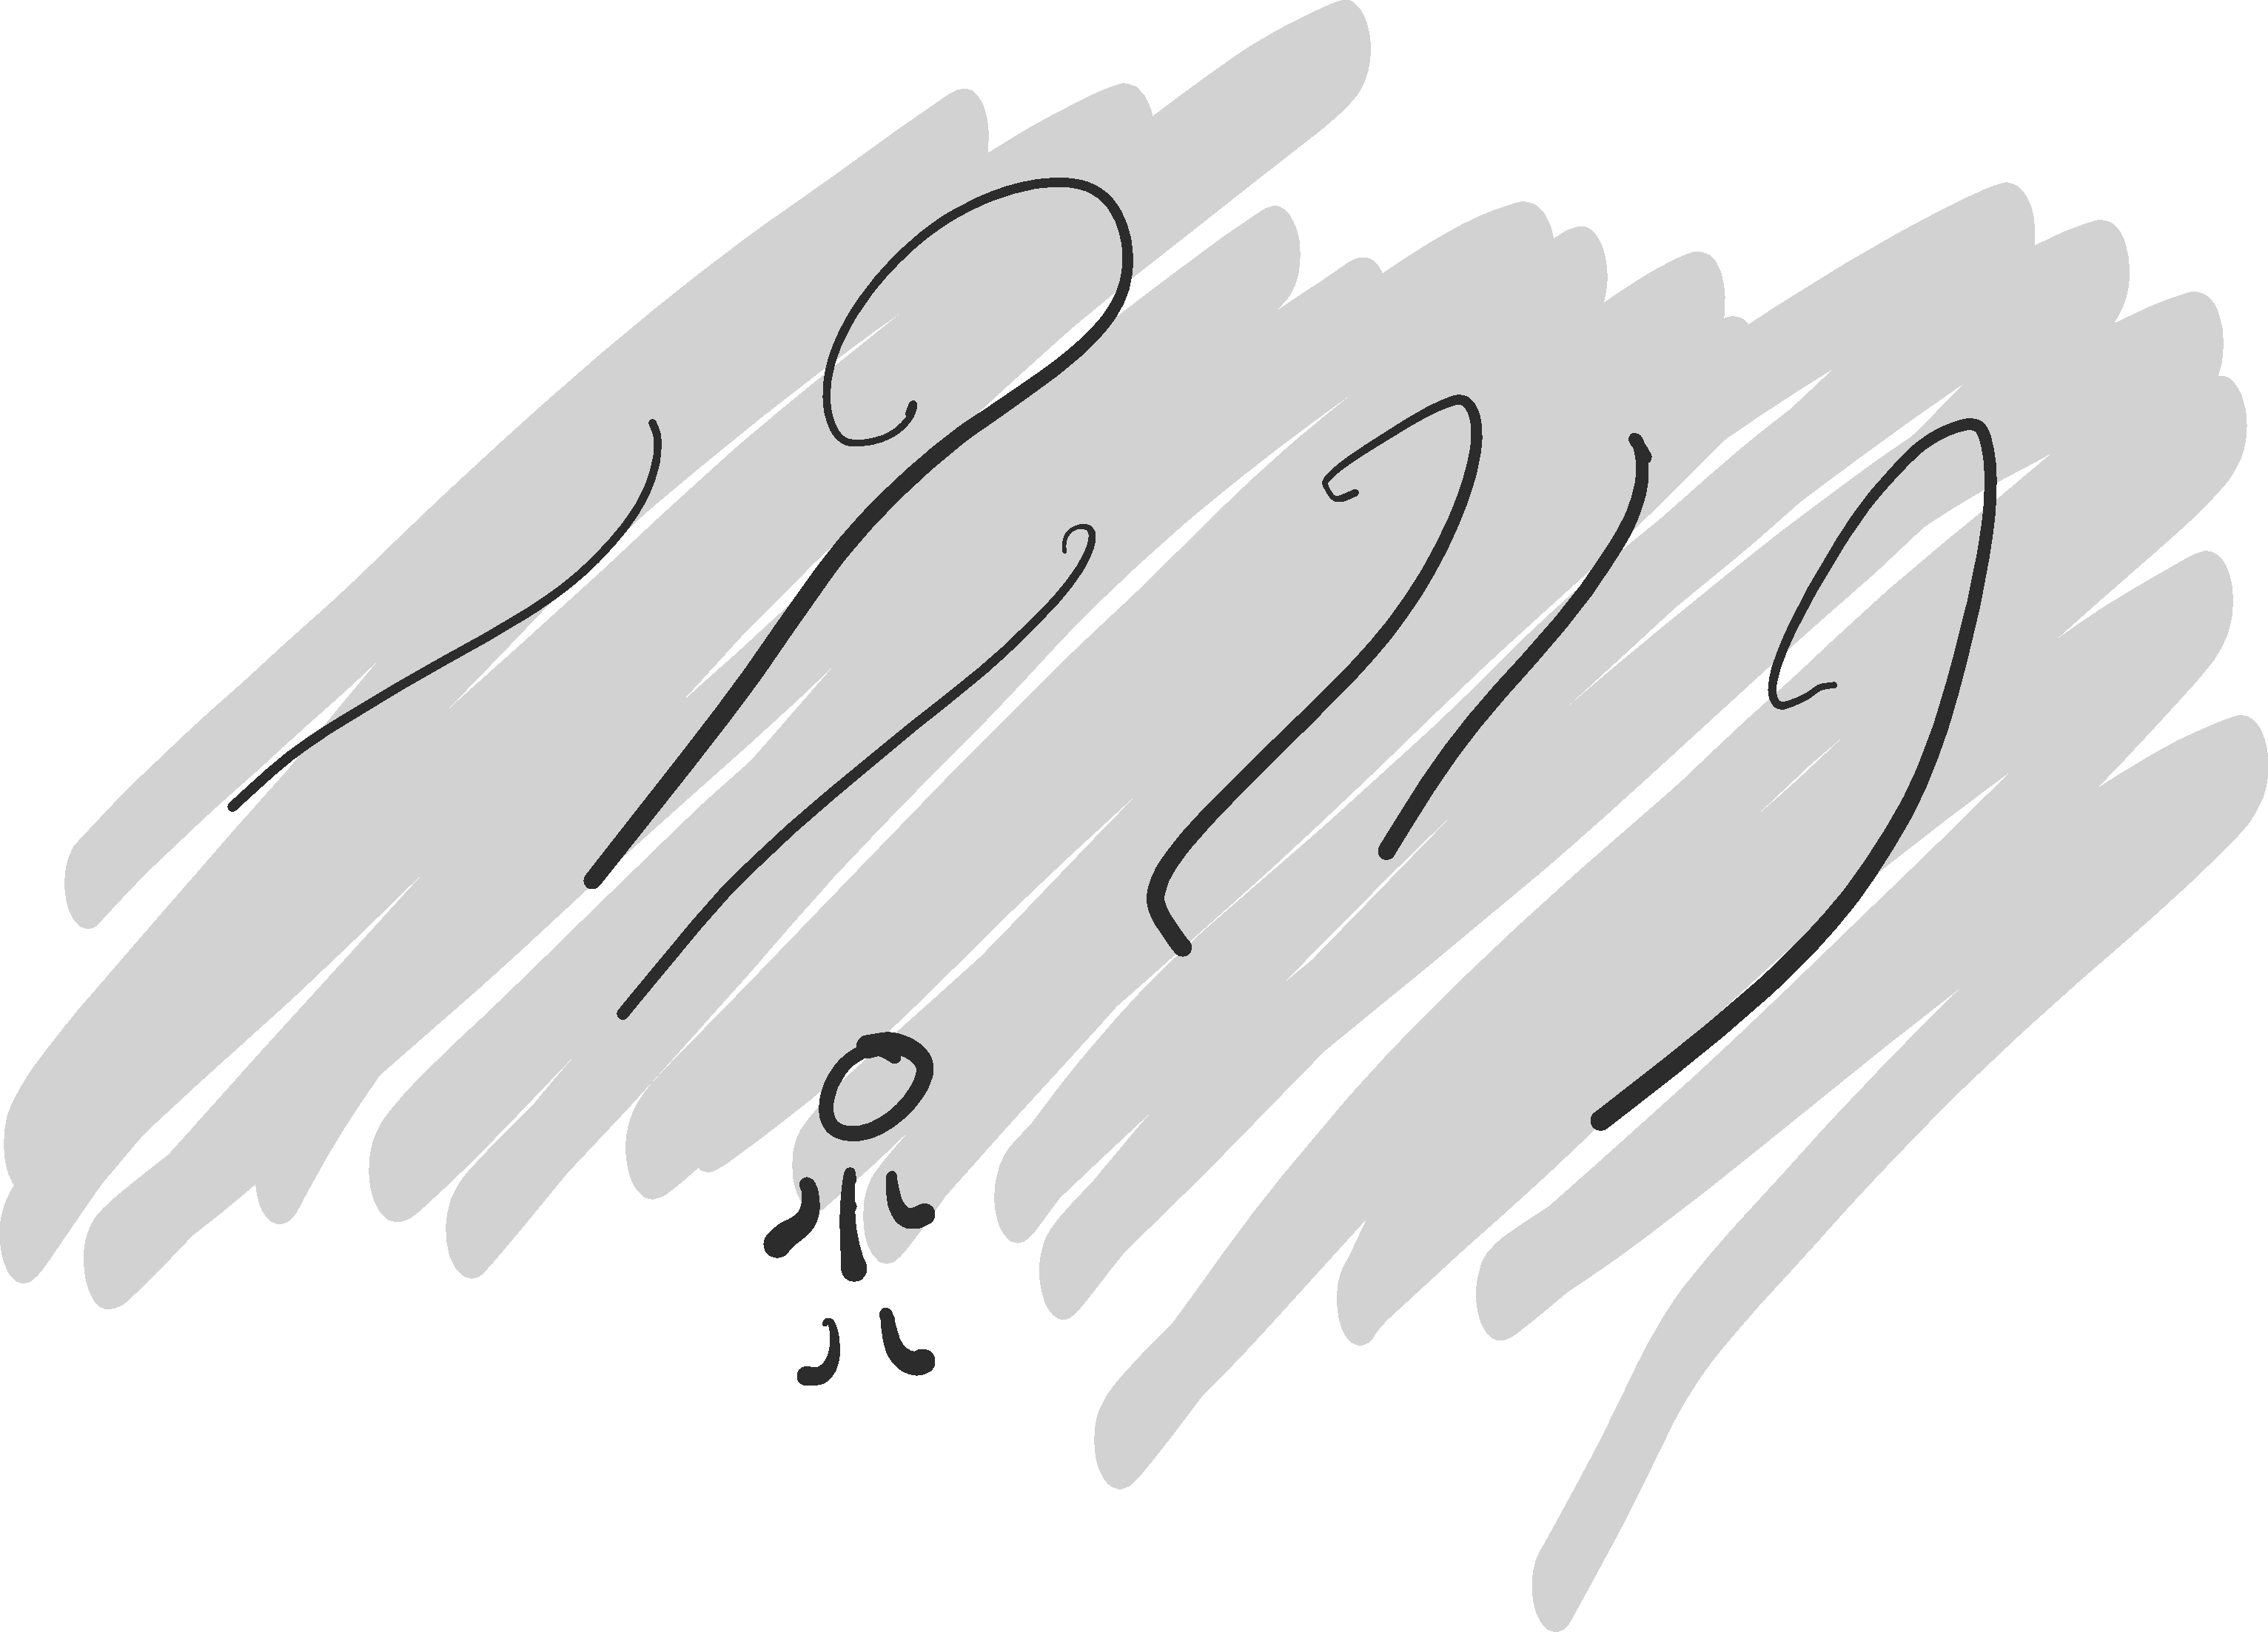
\includegraphics[width=0.3\textwidth]{img/cloud} \\
    $p_{\bm{P} = \text{wet}} = 0.5$
    }
  \end{tabular}
\end{center}

This setup looks familiar.
In the coin and die scenario, we had a pair of random variables that could each take on two values.
One random variable takes on each of its values with probability $\frac{1}{2}$.
the other random variable takes on one of its values with probability $\frac{9}{10}$ and the other with probability $\frac{1}{10}$.

The key difference is that precipitation and light are not independent.
Intuitively, we expect the wet and overcast conditions to be correlated and the dry and sunny conditions to be correlated.
For example, if it's raining we would be very surprised if it was sunny!

Let's look at how precipitation and light interact in our hypothetical scenario.
We will model the weather --- the combination of precipitation and light --- as a single random variable $\bm{W}$.
The weather can be in four possible states,
\begin{center}
 \begin{tabular}{c c || c | c }
 \multicolumn{2}{c}{\multirow{2}{*}{$\bm{W}$}} & \multicolumn{2}{c}{$\bm{P}$} \\
\multicolumn{2}{c}{} & rainy & dry \\ [0.5ex]
 \hline\hline
\multirow{10}{*}{$\bm{L}$} & sunny
& \makecell{
  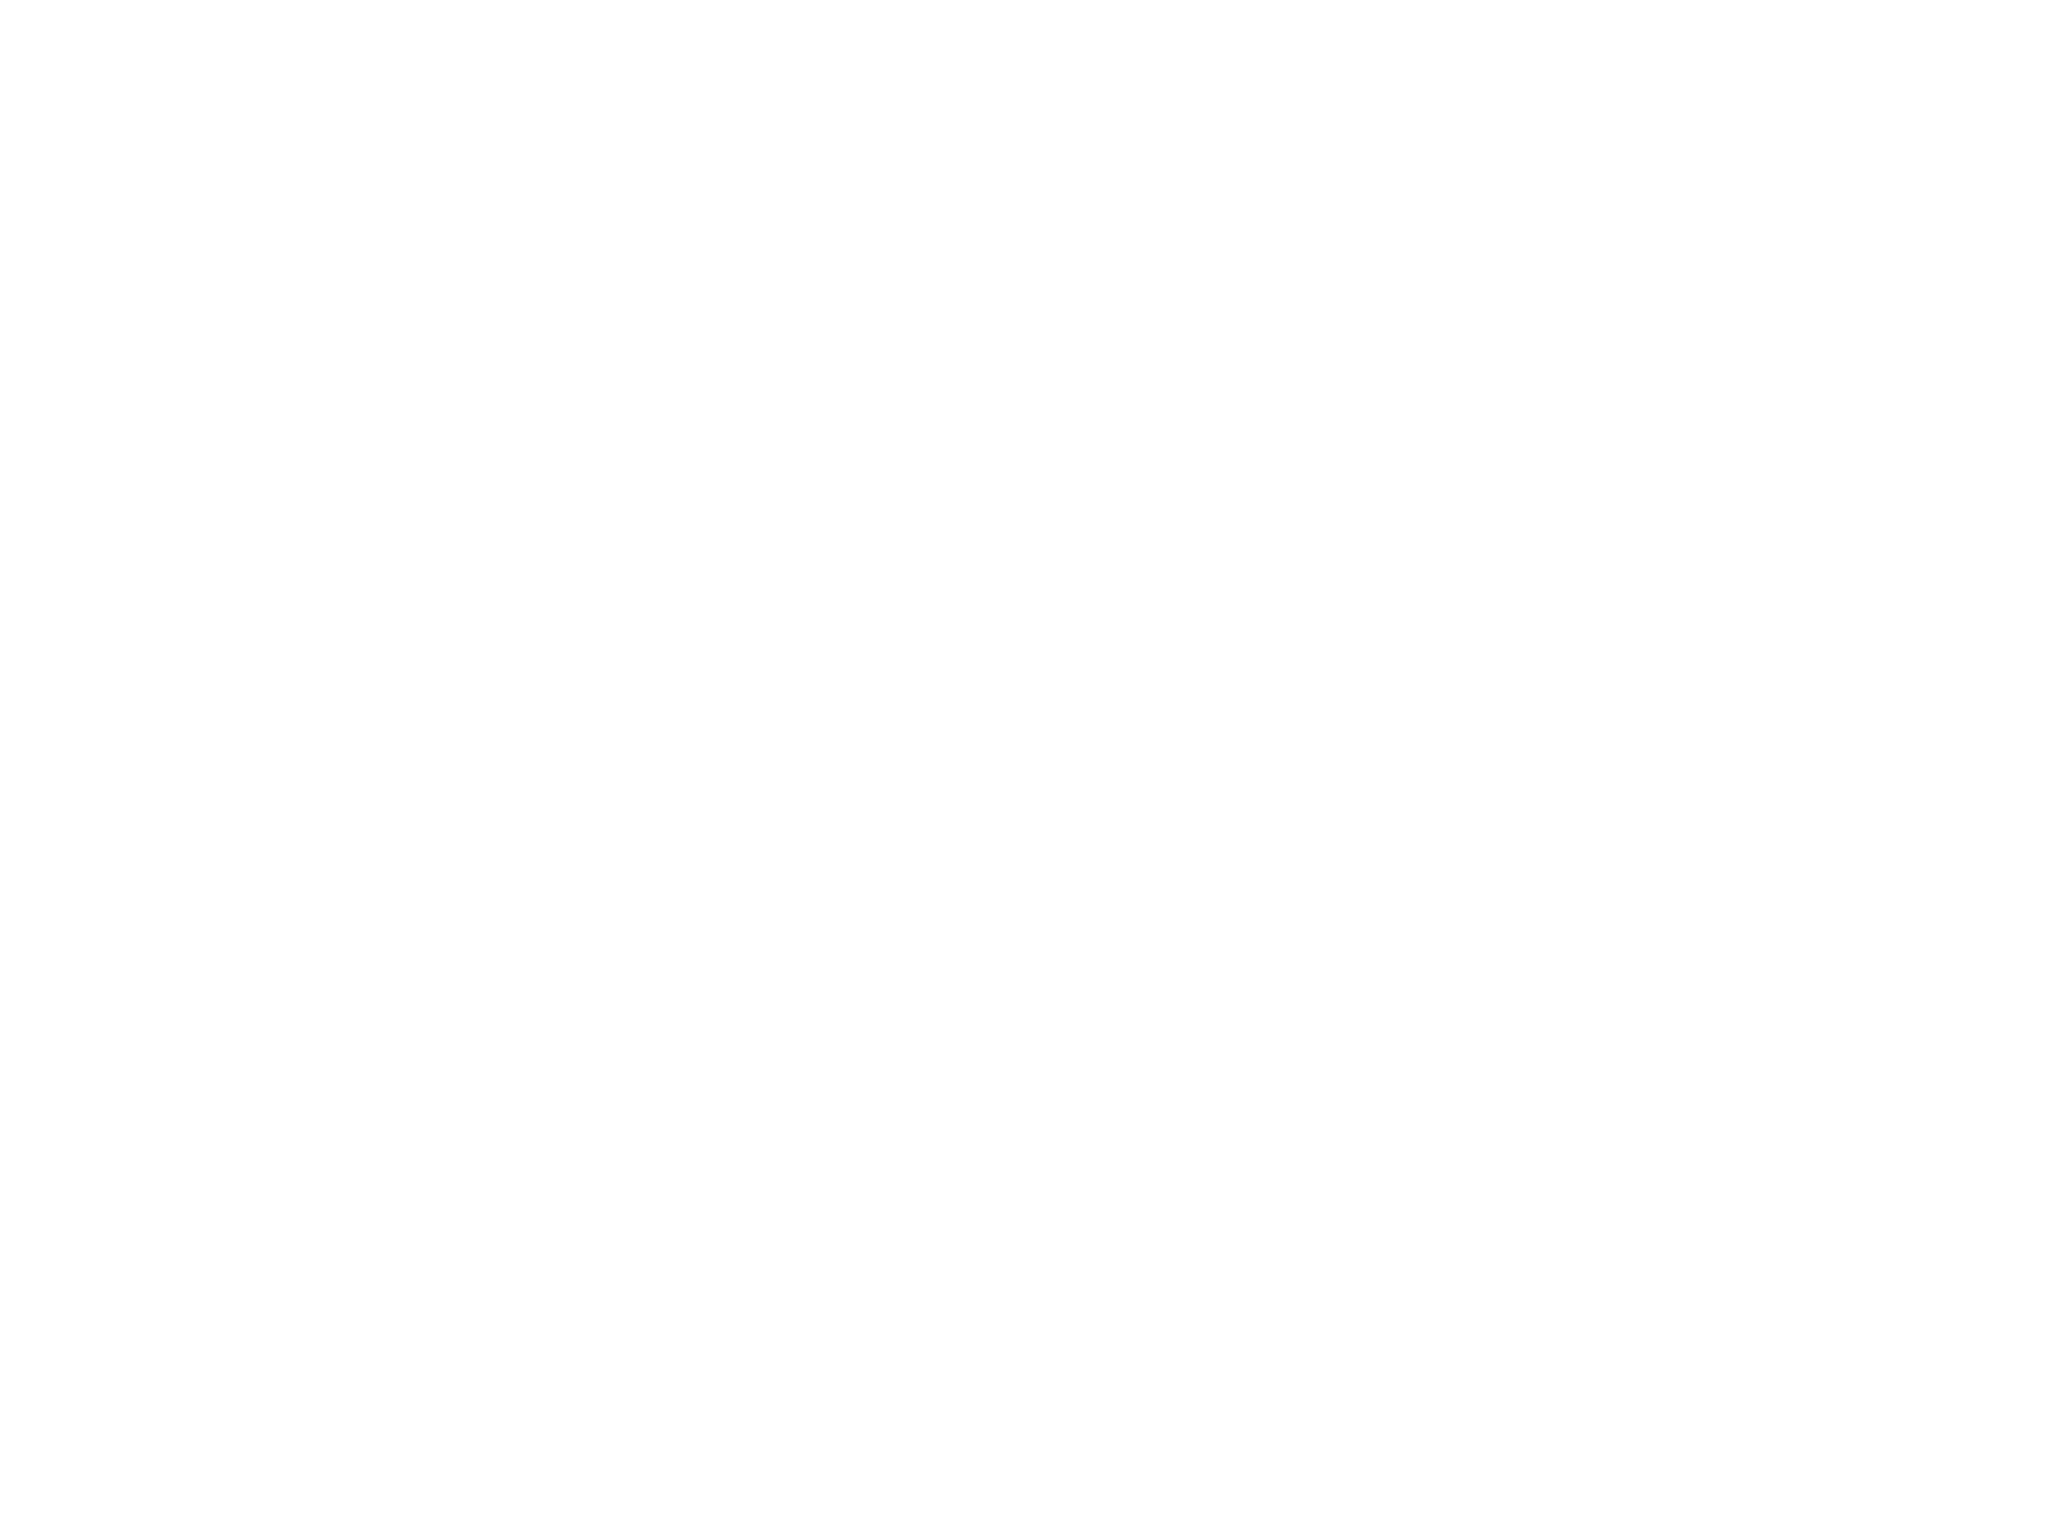
\includegraphics[trim= 0 0 0 0, clip, width=0.3\textwidth]{img/sun-rain} \\
  $\bm{W} = \text{``rainy, sunny''}$
  }
 & \makecell{
  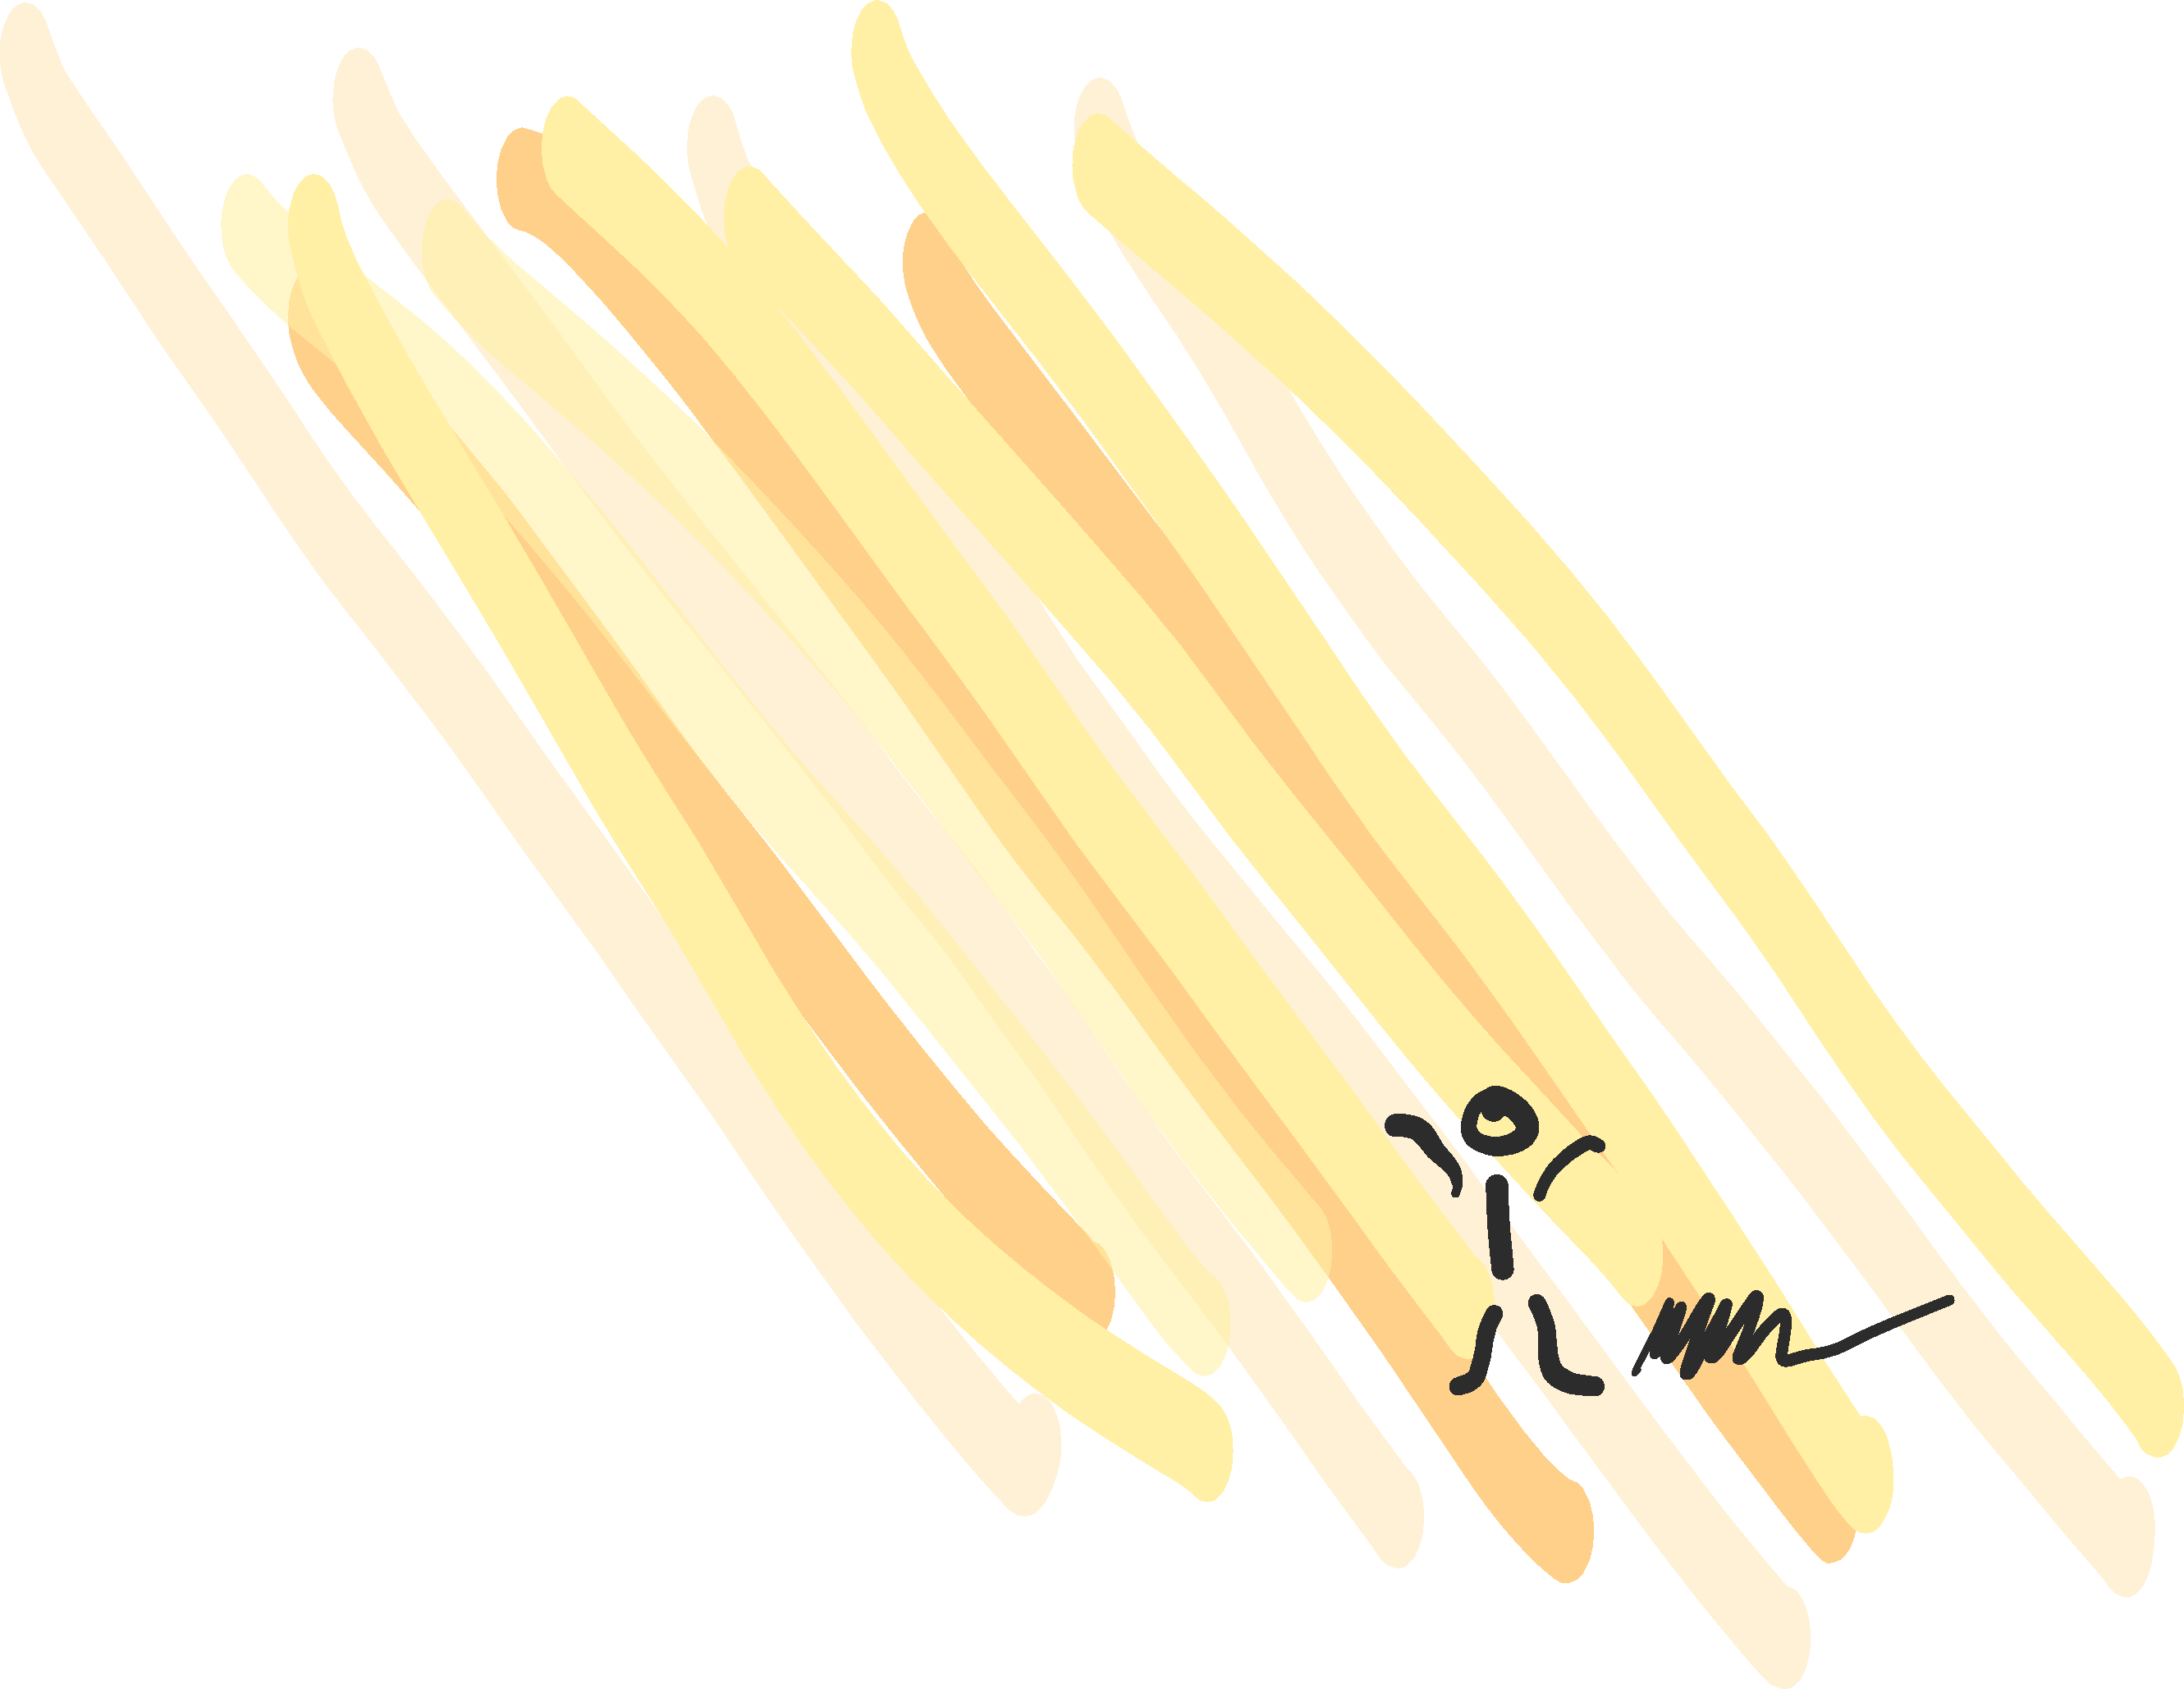
\includegraphics[trim= 0 0 0 0, clip, width=0.3\textwidth]{img/sun} \\
  $\bm{W} = \text{``dry, sunny''}$
  }
  \\
 \cline{2-4}
 & overcast
 & \makecell{
 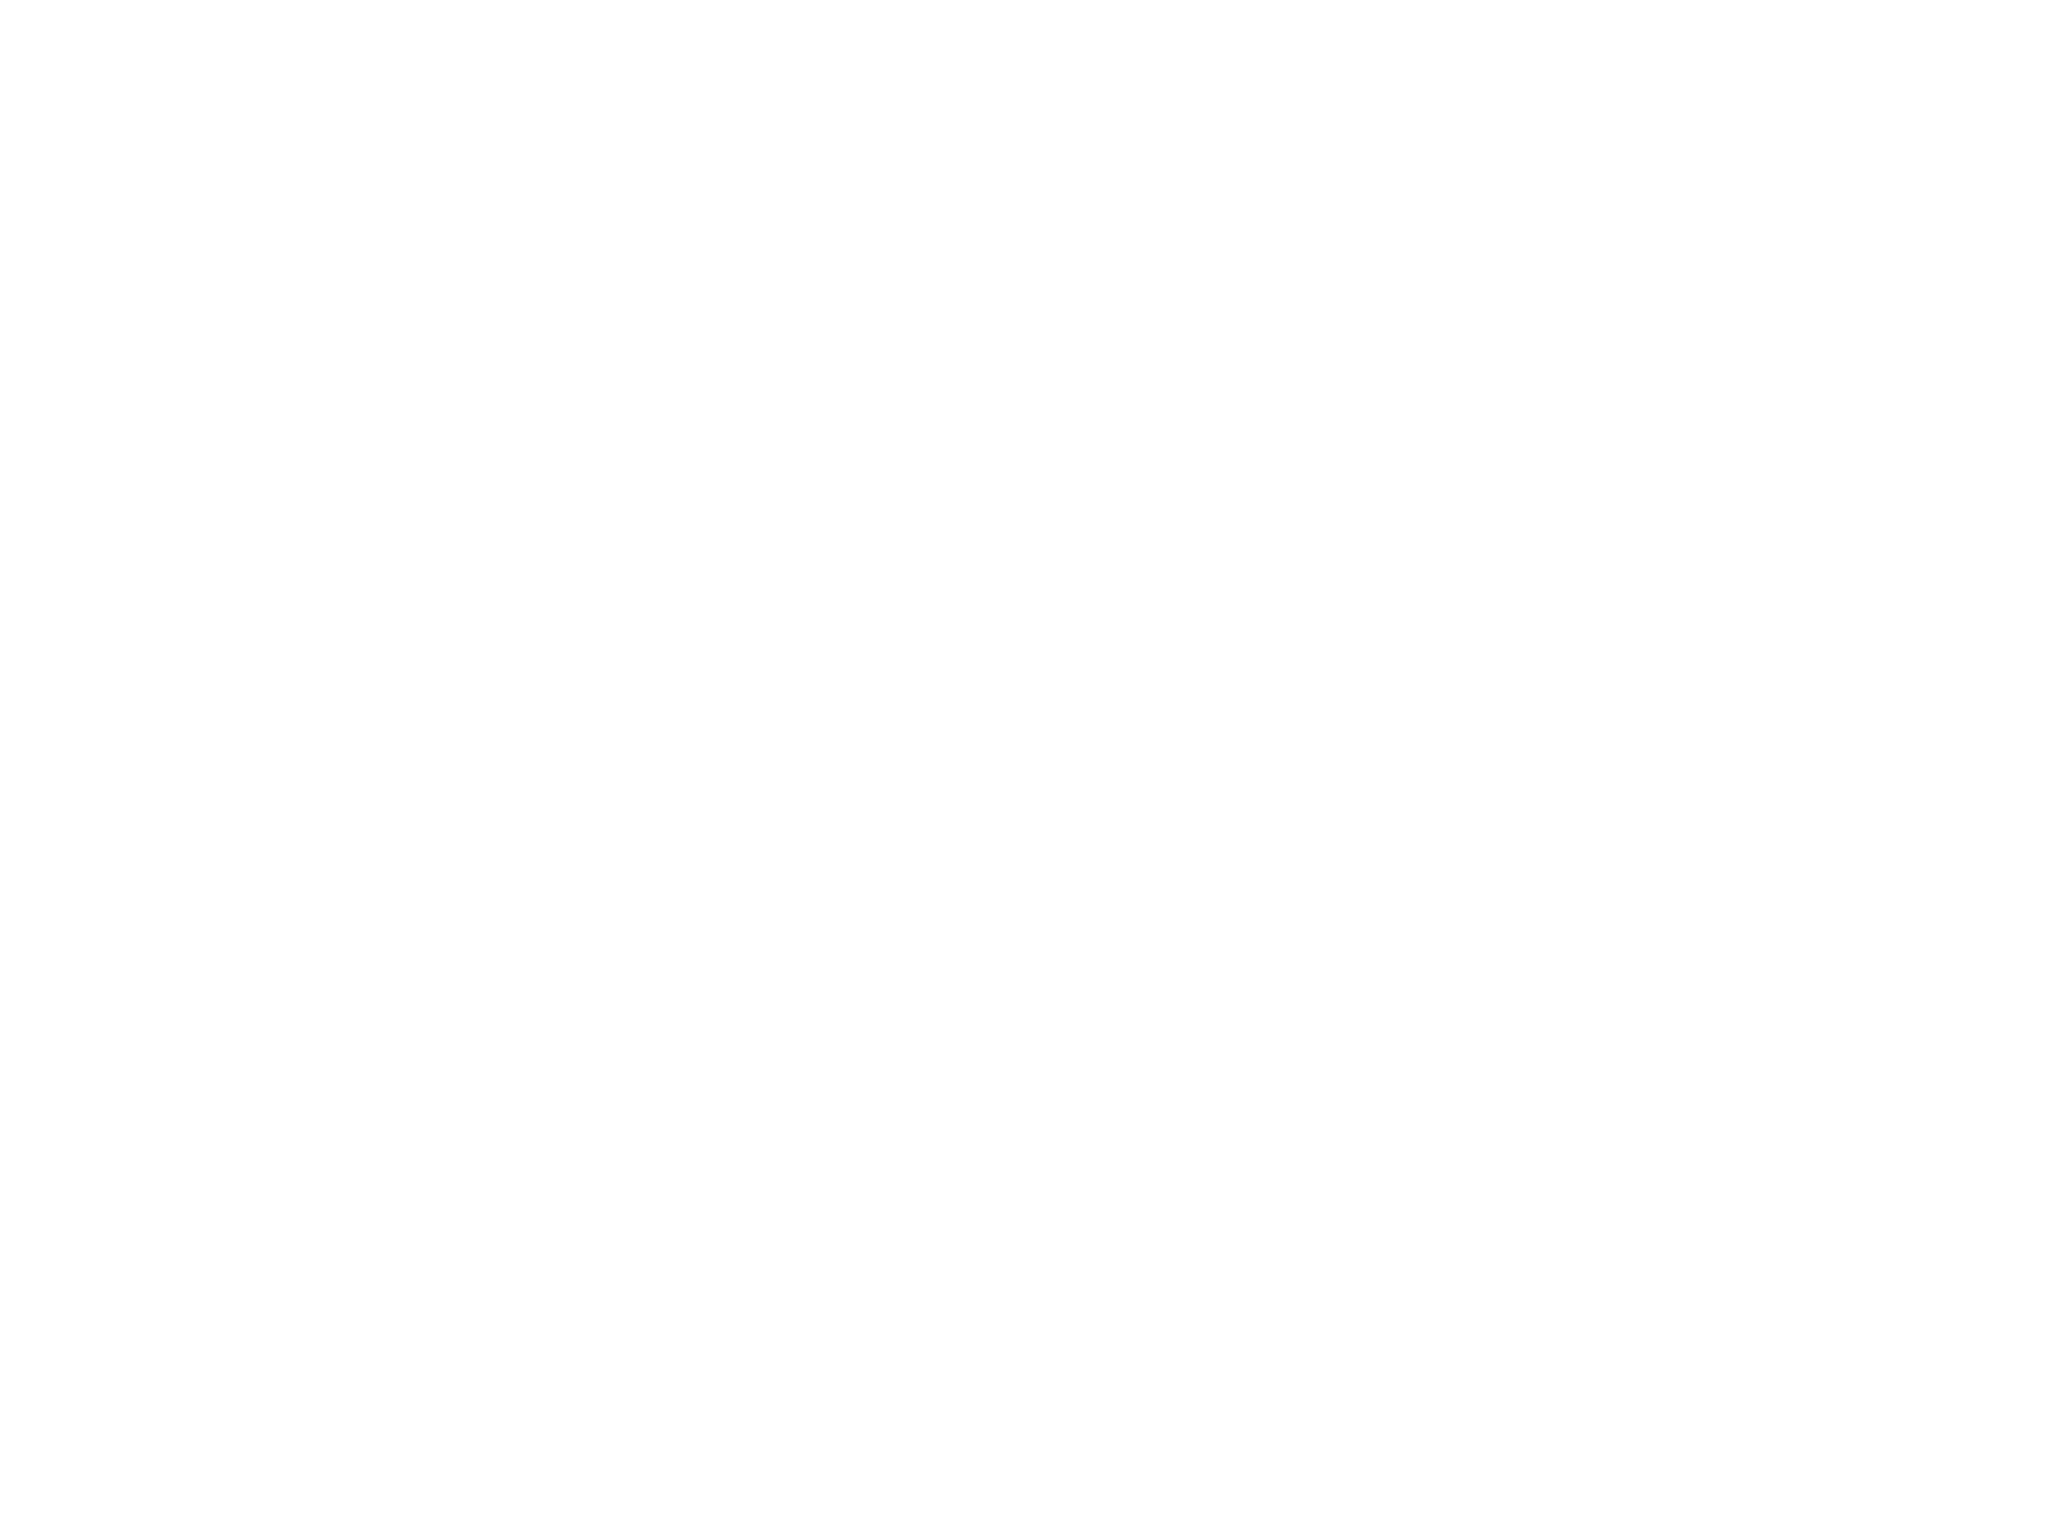
\includegraphics[trim= 0 0 0 0, clip, width=0.3\textwidth]{img/cloud-rain} \\
  $\bm{W} = \text{``rainy, overcast''}$}
 & \makecell{
 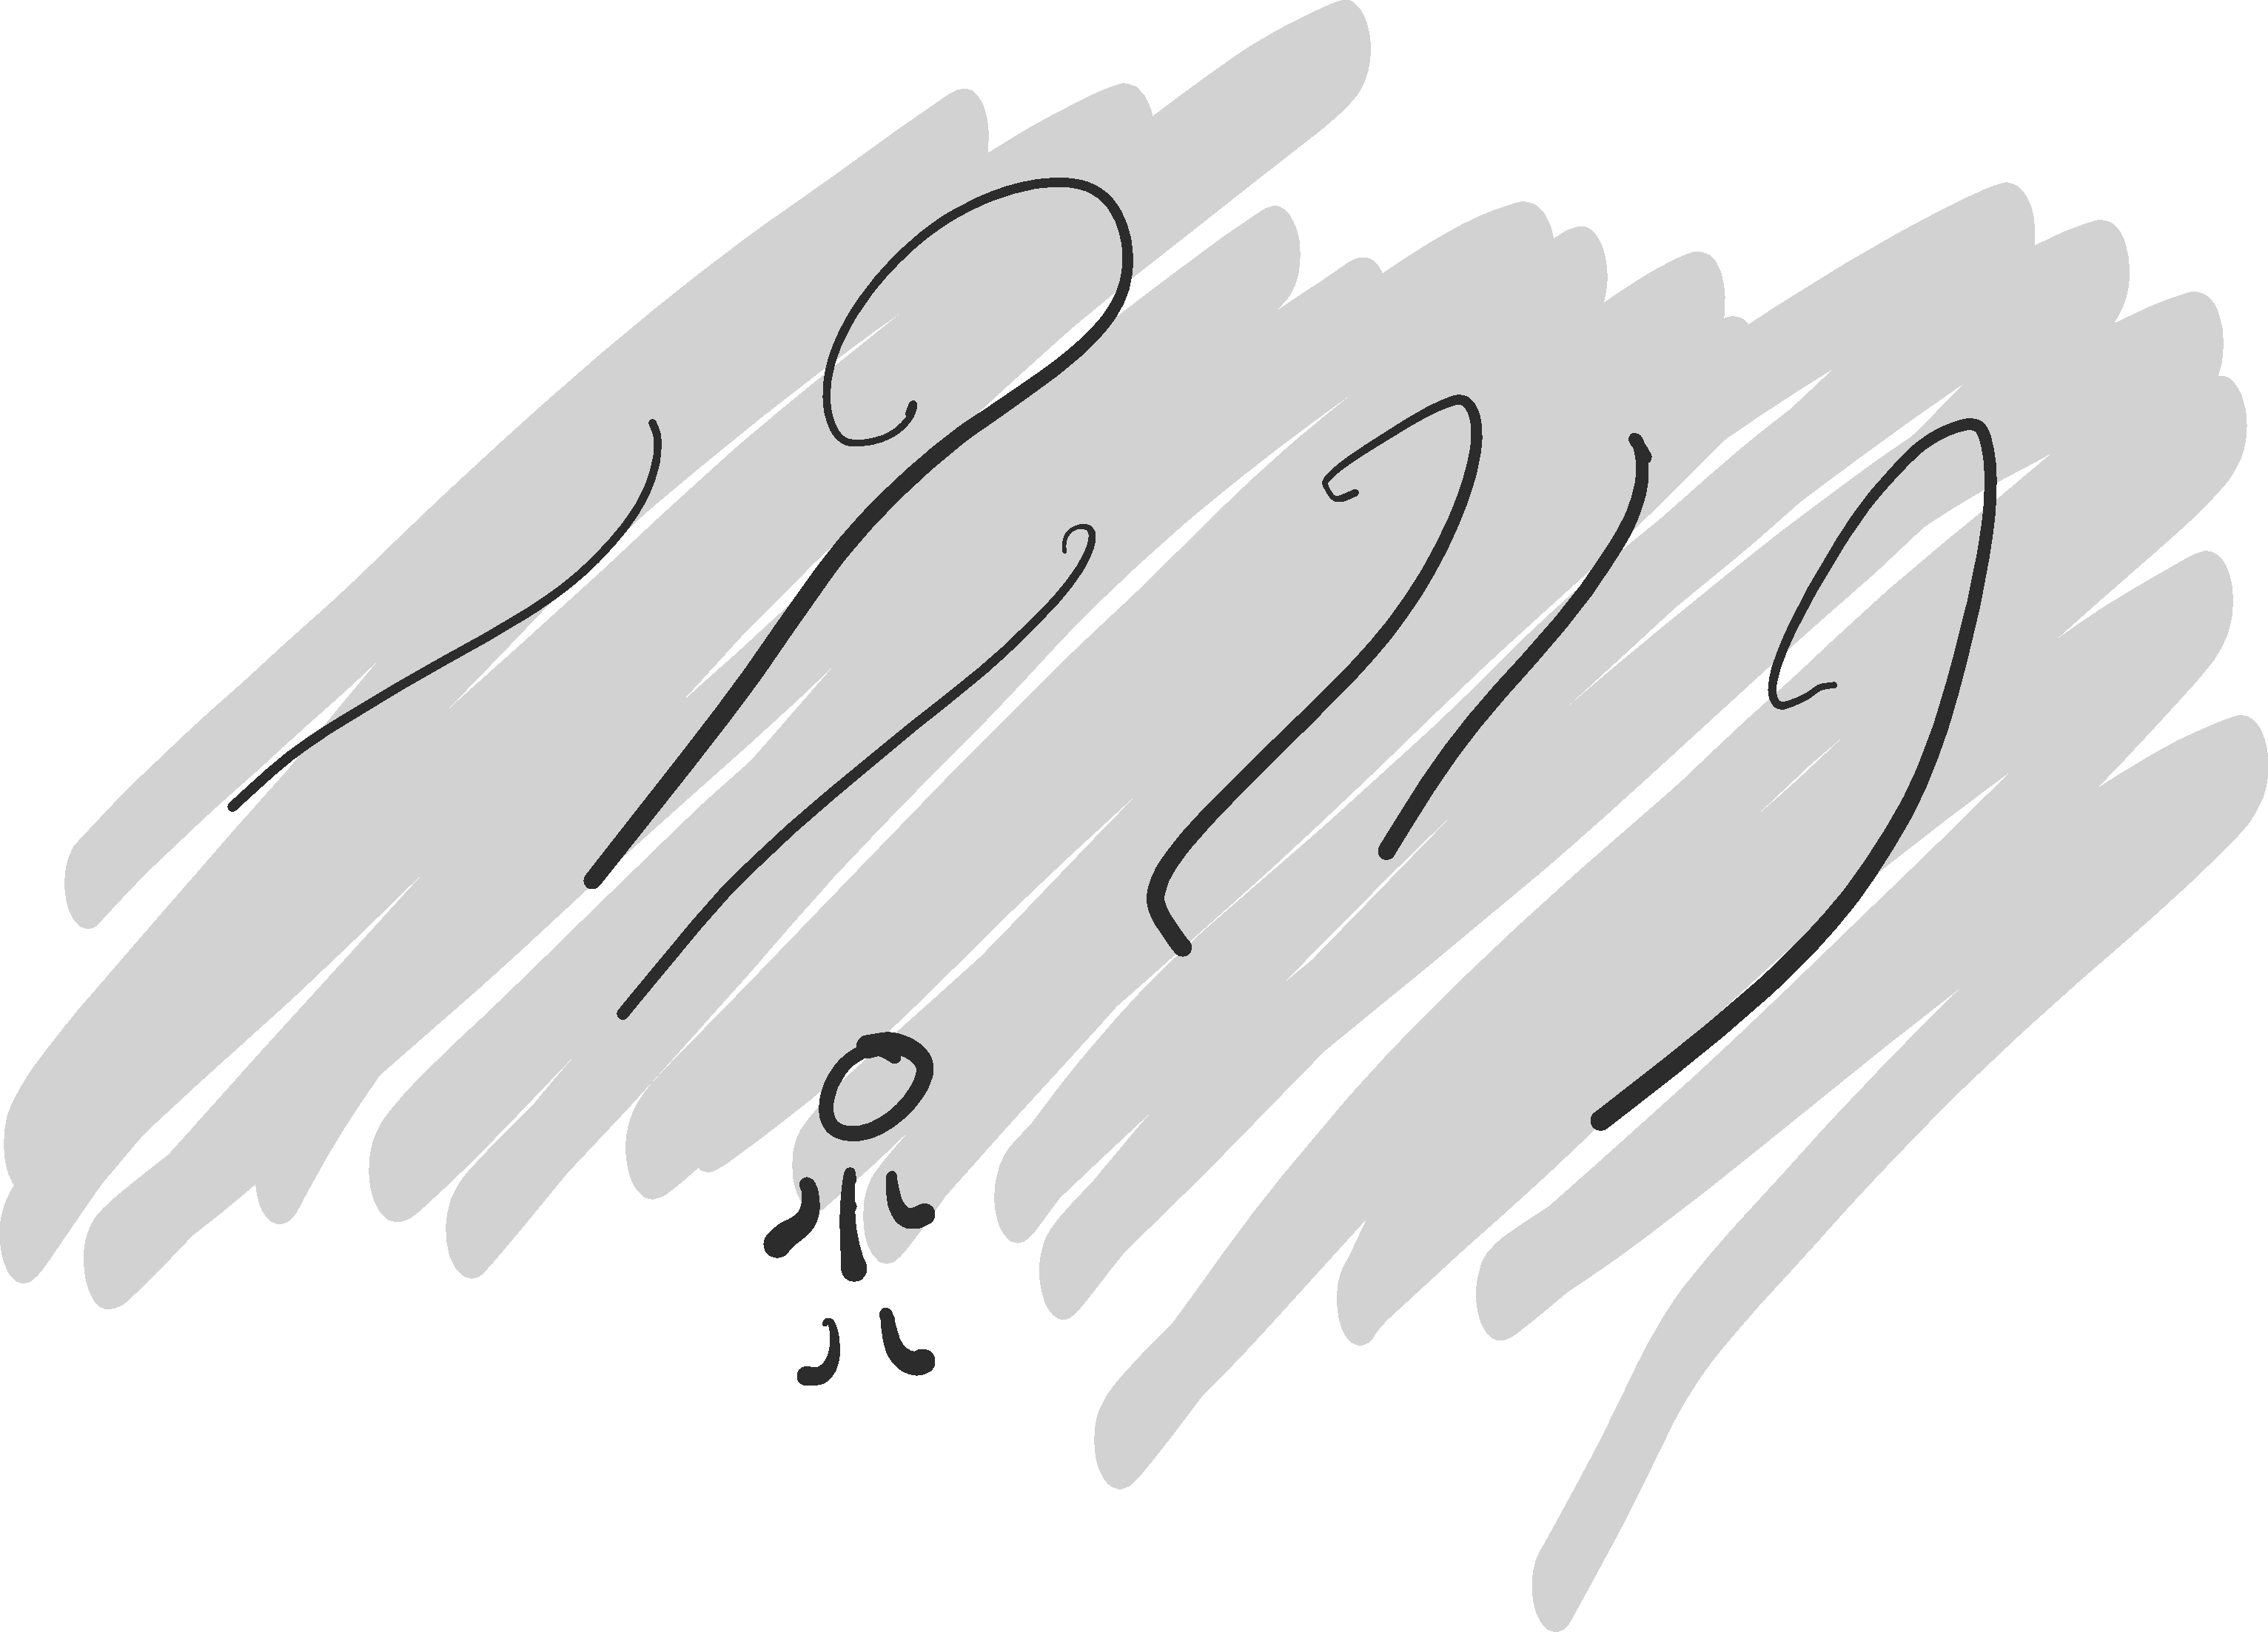
\includegraphics[trim= 0 0 0 0, clip, width=0.3\textwidth]{img/cloud} \\ $\bm{W} = \text{``dry, overcast''}$}
\end{tabular}
\end{center}

Because we are no longer operating under the assumption of independence, the probabilities of the four states of $\bm{W}$ can no longer be derived from the probability distributions of $\bm{P}$ (precipitation) and $\bm{L}$ (light).
Just as we took it at face value that in our scenario the probability of the sunny and cloudy condition are both $\frac{1}{2}$, we take the probability of each of the four possible states of $\bm{W}$ at face value as describing the particular scenario we are imagining.
(Of course, this is under the constraint that the marginal probabilities of $\bm{P}$ and $\bm{L}$ are consistent with what we stated before).
Let's define the probability distribution of $\bm{W}$ as follows,
\begin{center}
 \begin{tabular}{c c || c | c || c}
 \multicolumn{2}{c}{\multirow{2}{*}{$\bm{W}$}} & \multicolumn{2}{c}{$\bm{L}$} & {}\\
\multicolumn{2}{c}{} & sunny & overcast & sum \\ [0.5ex]
 \hline\hline
\multirow{2}{*}{$\bm{P}$} & wet & 0.005 & 0.095 & 0.1 \\
 \cline{2-5}
 & dry & 0.495 & 0.405 & 0.9 \\
 \hline\hline
  {} & sum & 0.5 & 0.5 & 1 \\ [1ex]
\end{tabular}.
\end{center}

The best way to get a feel for the distribution of $\bm{W}$ is to look at conditional probabilities.
For example, here's the probability that we observe the sunny weather given we know that it's wet outside,
\begin{align*}
P(\bm{L} = \text{sunny} | \bm{P} = \text{wet}) &= 0.05.
\end{align*}

Although we won't elaborate on it, calculating such conditional probabilities from the table above is very straightforward.
Let's look through the rest of the rest of the conditional probabilities we can calculate.

Consider
\begin{align*}
  P(\bm{L} = \text{sunny} | \bm{P} = \text{dry}) &= 0.55 \\
  P(\bm{L} = \text{sunny}) &= 0.5 \\
  P(\bm{L} = \text{sunny} | \bm{P} = \text{wet}) &= 0.05.
\end{align*}
Here, we see that the probability of observing sunny weather is greatest if we know that it's dry outside and very small if we know that it's wet outside.

Likewise,
\begin{align*}
P(\bm{L} = \text{overcast} | \bm{P} = \text{wet}) &= 0.95 \\
P(\bm{L} = \text{overcast}) &= 0.5 \\
P(\bm{L} = \text{overcast} | \bm{P} = \text{dry}) &= 0.45.
\end{align*}
The probability of observing overcast weather is greatest if we know that it's wet outside and less if we know that it's dry outside.

Similarly,
\begin{align*}
P(\bm{P} = \text{wet} | \bm{L} = \text{overcast}) &= 0.19 \\
P(\bm{P} = \text{wet}) &= 0.1 \\
P(\bm{P} = \text{wet} | \bm{L} = \text{sunny}) &= 0.01.
\end{align*}
The probability of observing wet weather is greatest if we know it's overcast outside and least if we know it's sunny outside.

Finally,
\begin{align*}
P(\bm{P} = \text{dry} | \bm{L} = \text{sunny}) &= 0.99 \\
P(\bm{P} = \text{dry}) &= 0.9 \\
P(\bm{P} = \text{dry} | \bm{L} = \text{overcast}) &= 0.81.
\end{align*}
The probability of observing dry weather is greatest if we know it's sunny outside and least if we know it's overcast.

Armed with a good understanding of the probability distribution of our weather $\bm{W}$, we're ready to talk entropy and information.
We can calculate entropy of a random variable whose distribution we know using Equation \ref{eqn:shannon}.
Let's do that for $\bm{W}$,
\begin{align*}
S_{\text{weather}}
&=
H(\bm{W}) \\
&=
- 0.005 \times \log_2(0.005)
+ - 0.095 \times \log_2(0.095)
- 0.495 \times \log_2(0.495)
+ - 0.405 \times \log_2(0.405) \\
&\approx 1.391
\end{align*}
for $\bm{L}$,
\begin{align*}
  S_{\text{light}}
  &=
  H(\bm{L}) \\
  &=
  - 0.5 \times \log_2(0.5)
  + - 0.5 \times \log_2(0.5) \\
  &= 1
\end{align*}
and, finally, for $\bm{P}$,
\begin{align*}
  S_{\text{precipitation}}
  &=
  H(\bm{P}) \\
  &=
  - 0.1 \times \log_2(0.1)
  + - 0.9 \times \log_2(0.9) \\
  &\approx 0.469.
\end{align*}

Just like for the die and the coin, $S_{\text{light}} > S_{\text{precipitation}}$.
Like before, this makes sense because we can make a better guess about precipitation (it is wet infrequently) than about light conditions (it is overcast or sunny with equal probability).

Here's the shocker,
\begin{align*}
S_{\text{weather}}
\not{=}
S_{\text{light}} + S_{\text{precipitation}}
\end{align*}
In fact, $1.391 < 1.469$, so
\begin{align*}
S_{\text{weather}}
<
S_{\text{light}} + S_{\text{precipitation}}.
\end{align*}
How can our uncertainty about the weather as an entire system be less than our uncertainty about its constituent parts?
The answer is that some entropy is shared between $\bm{L}$ and $\bm{P}$.
The situation looks like this.
\begin{center}
  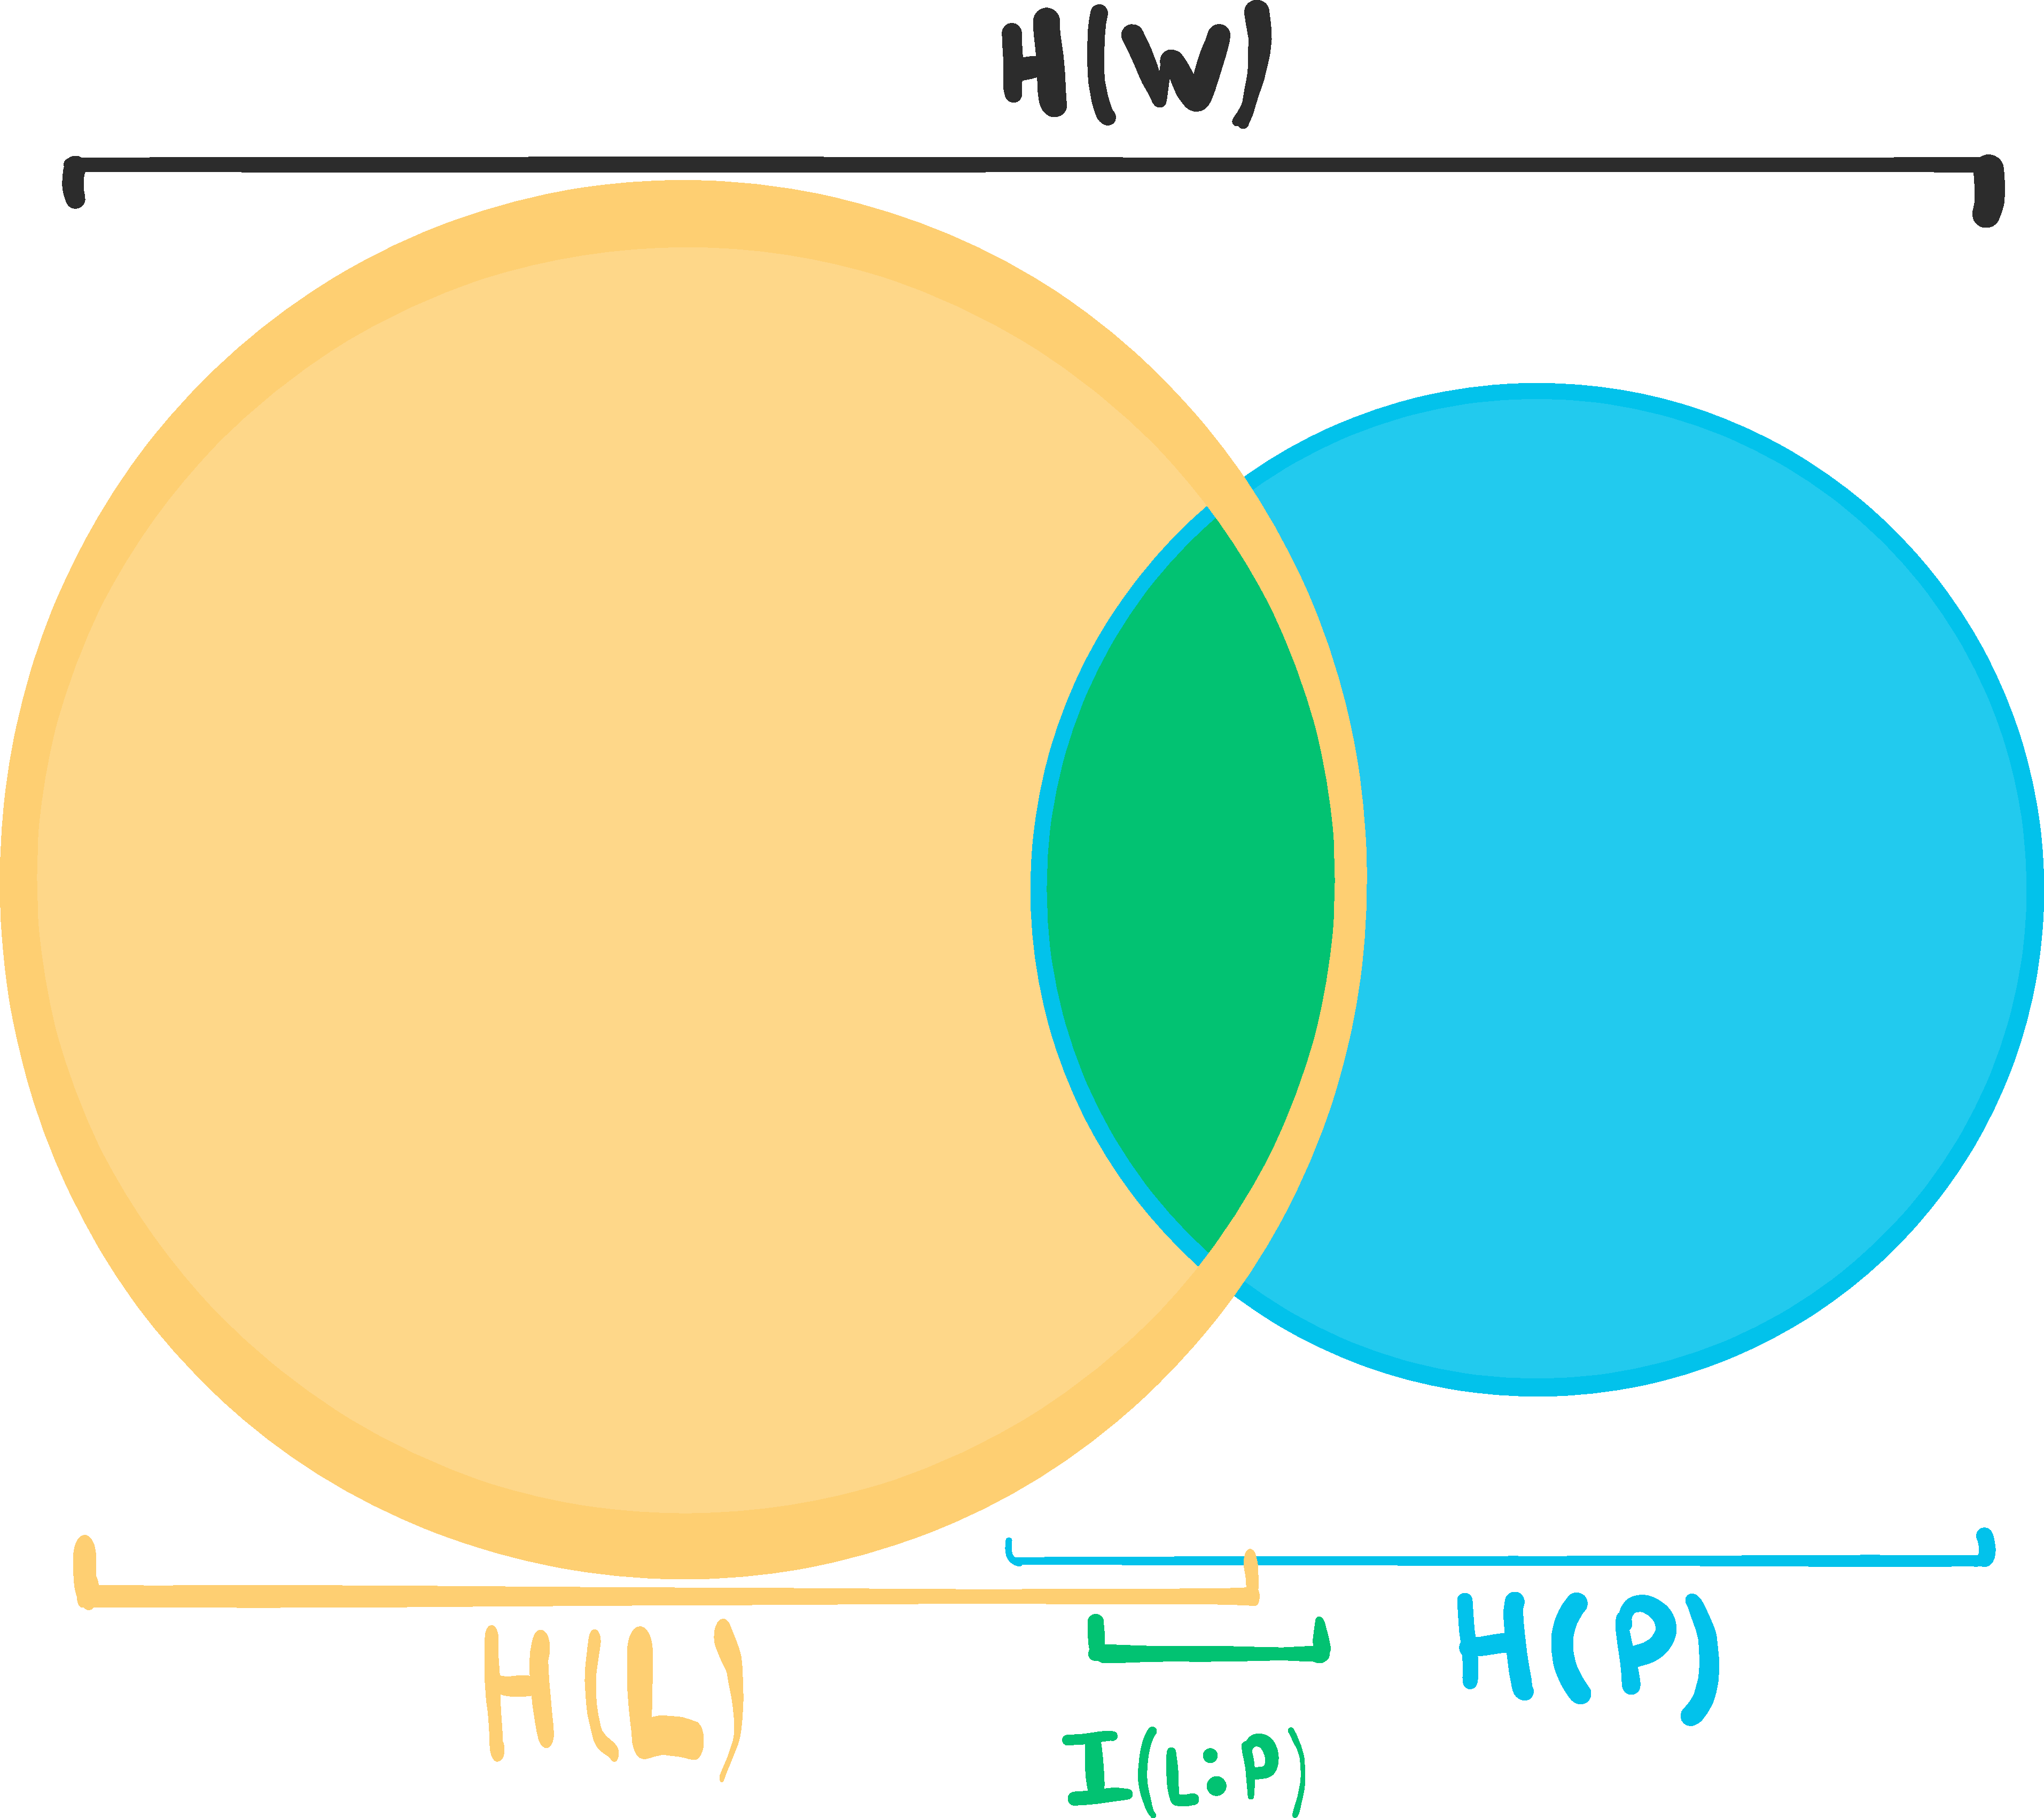
\includegraphics[trim= 0 0 0 0, clip, width=0.6\textwidth]{img/venn}
\end{center}
The green silver in the middle of this venn diagram is the entropy shared between $\bm{L}$ and $\bm{P}$.
I denoted that sliver $I( \bm{L} : \bm{P})$.
(Shared entropy is symmetric, so it would be just as valid to denote it $I( \bm{P} : \bm{L})$).
In total, the shaded area represents the entropy of the entire system $H(\bm{W})$.
If we stepped out the door to observe the state of the weather all at once, all of that entropy would go away.
\begin{center}
  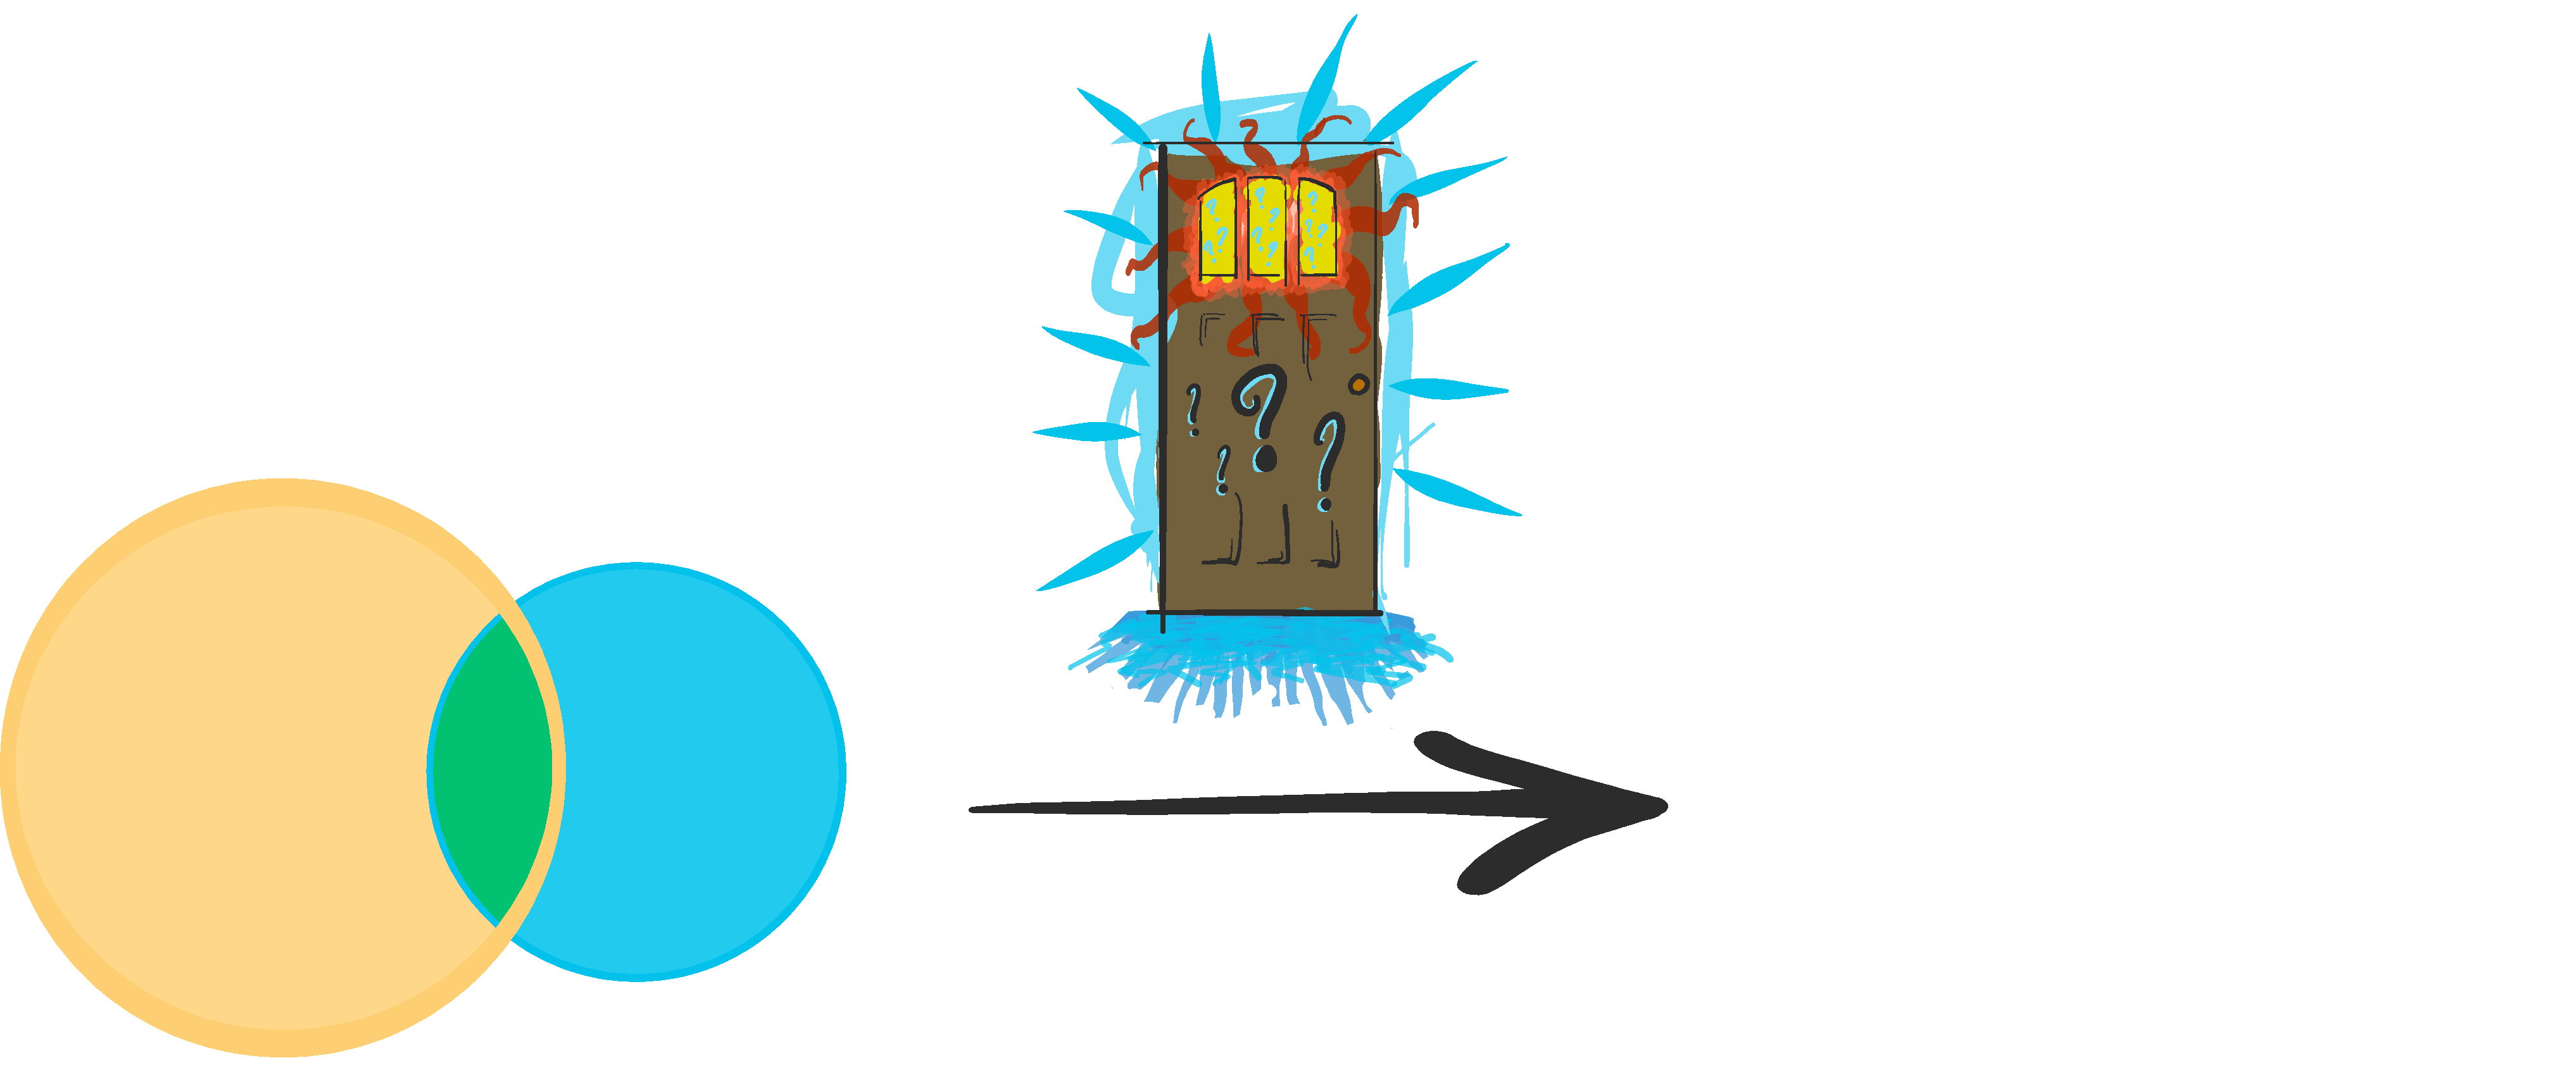
\includegraphics[trim= 0 0 0 0, clip, width=0.9\textwidth]{img/mystery-door-peek}
\end{center}


This idea of sharing entropy has an interesting implication.
Say we had a rain meter that tells us the precipitation conditions.
Knowing the precipitation conditions removes all the blue uncertainty ($H(\bm{P})$) from our diagram, taking some of the yellow uncertainty ($H(\bm{L})$) with it.
\begin{center}
  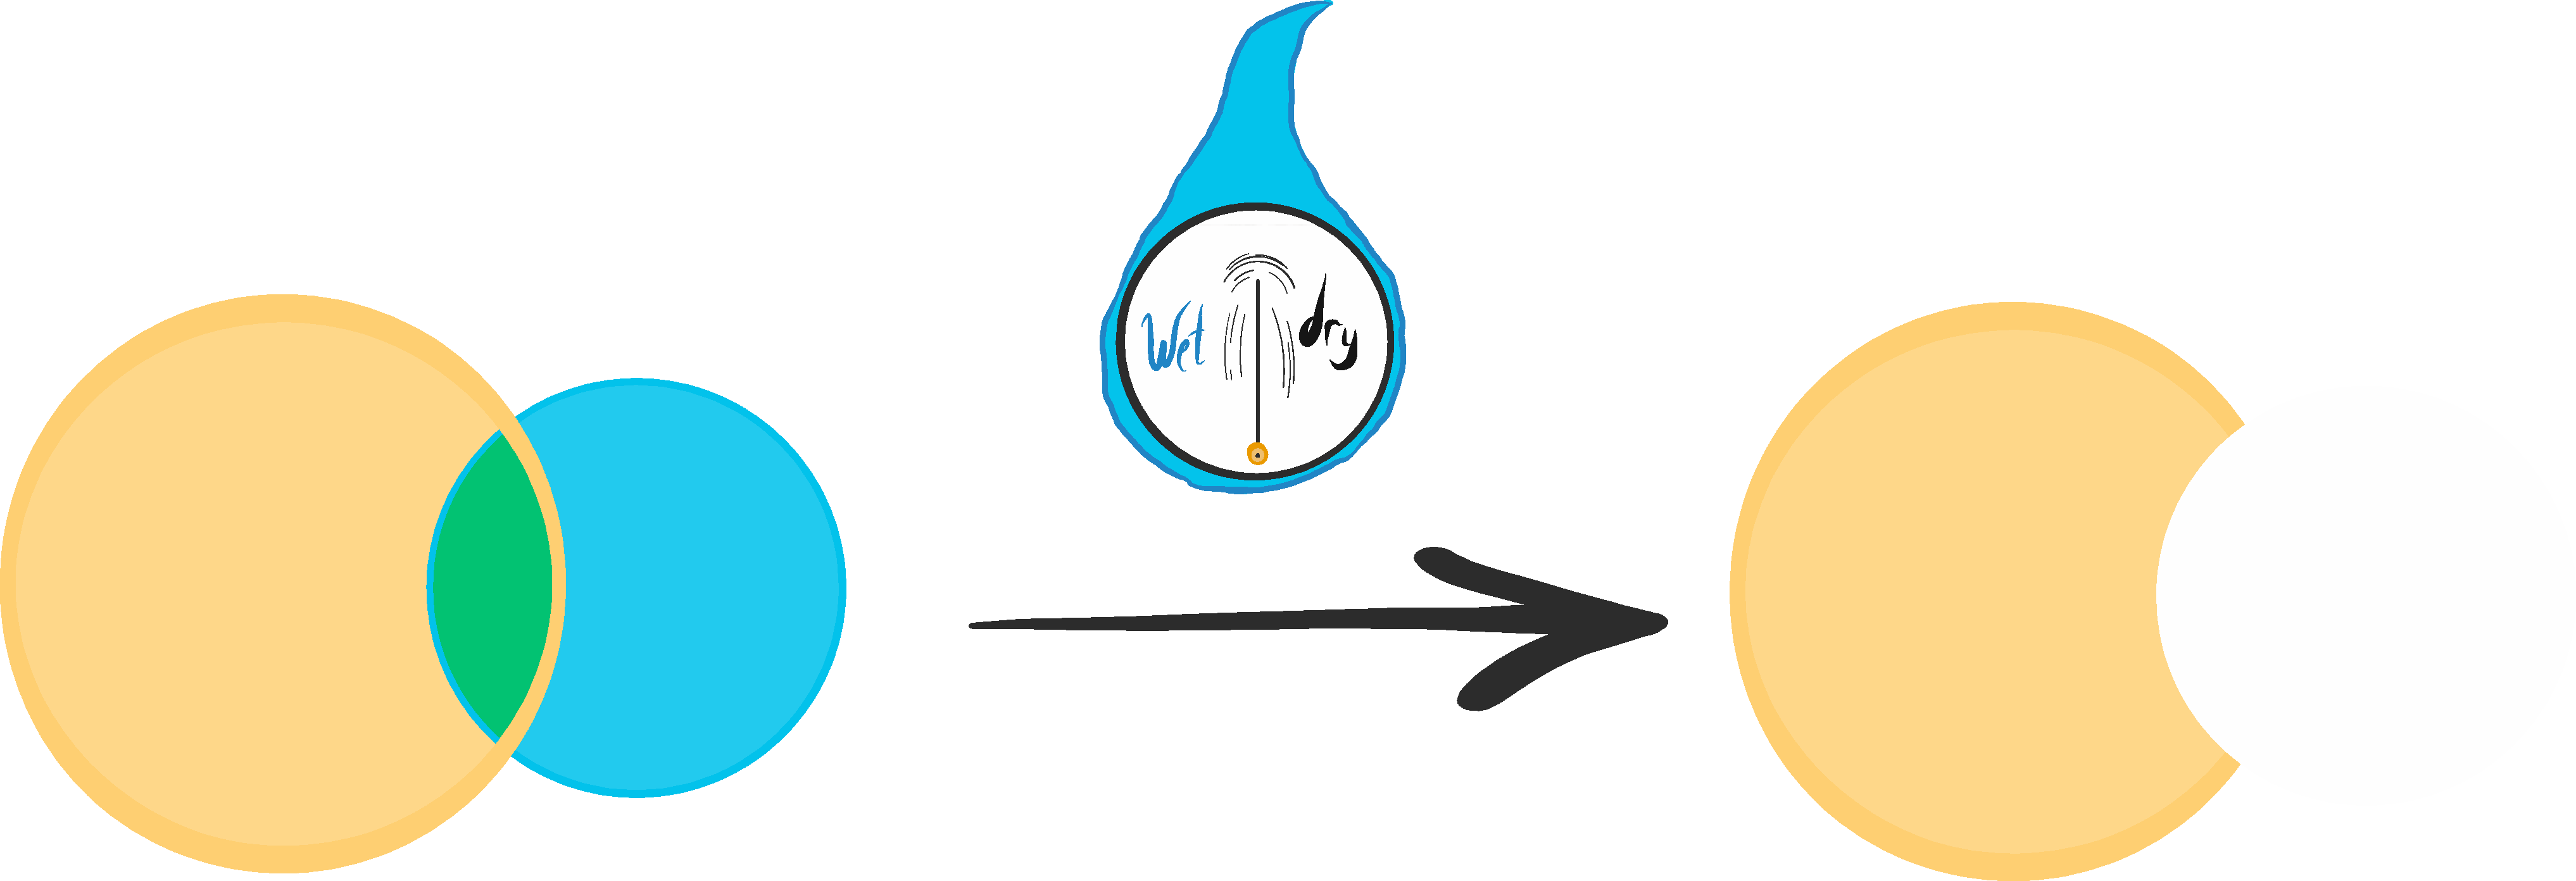
\includegraphics[trim= 0 0 0 0, clip, width=0.9\textwidth]{img/rain-meter-peek}
\end{center}
Thus, we would expect our uncertainty about light conditions to be reduced by knowing the precipitation conditions.
This is indeed the case.
We can calculate this directly!

To calculate the entropy after peeking at the rain meter, we need to calculate our uncertainty as to the light condition after we observe the rain meter.
There are two outcomes from looking at the rain meter --- we learn it's wet outside or we learn it's dry outside.
Remember the conditional probabilities we reviewed?
To calculate entropy given a particular precipitation state, we proceed as usual with Shannon's equation but substitute probabilities conditional on the precipitation state we observed for unconditional probabilities.

If we find it's wet outside, we calculate
\begin{align*}
H(\bm{L} | \bm{P} = \text{wet})
&=
- P(\bm{L} = \text{sunny} | \bm{P} = \text{wet}) \times \log_2(P(\bm{L} = \text{sunny} | \bm{P} = \text{wet})) \\
&+ - P(\bm{L} = \text{overcast} | \bm{P} = \text{wet}) \times \log_2(P(\bm{L} = \text{overcast} | \bm{P} = \text{wet})) \\
\approx&
- 0.05 \times \log_2(0.05) + - 0.95 \times \log_2(0.95) \\
\approx& 0.286.
\end{align*}
If we find it's dry outside, we calculate
\begin{align*}
H(\bm{L} | \bm{P} = \text{dry})
=&
- P(\bm{L} = \text{sunny} | \bm{P} = \text{dry}) \times \log_2(P(\bm{L} = \text{sunny} | \bm{P} = \text{dry})) \\
&+  - P(\bm{L} = \text{overcast} | \bm{P} = \text{dry}) \times \log_2(P(\bm{L} = \text{overcast} | \bm{P} = \text{dry})) \\
=&
- 0.55 \times \log_2(0.55) + - 0.45 \times \log_2(0.45) \\
\approx& 0.993.
\end{align*}

From these results, we can calculate the expected entropy of $\bm{L}$ given observation of $\bm{P}$.
We denote this quantity as $H(\bm{L}|\bm{P})$.
We calculate $H(\bm{L}|\bm{P})$ by taking an average of $H(\bm{L} | \bm{P} = \text{dry})$ and $H(\bm{L} | \bm{P} = \text{wet})$, weighted by the probabilities $P(\bm{P} = \text{wet})$ and $P(\bm{P} = \text{dry})$,
\begin{align*}
H(\bm{L} | \bm{P})
=&
P(\bm{P} = \text{wet}) \times H(\bm{L} | \bm{P} = \text{wet}) \\
&+ P(\bm{P} = \text{dry}) \times H(\bm{L} | \bm{P} = \text{dry}) \\
\approx& 0.1 \times [ - 0.05 \times \log_2(0.05) + - 0.95 \times \log_2(0.95) ] \\
&+ 0.9 \times [ - 0.55 \times \log_2(0.55) + - 0.45 \times \log_2(0.45) ] \\
\approx& 0.922.
\end{align*}

Recall that information is the difference between entropies.
Thus, we can think of the shared entropy between $\bm{P}$ and $\bm{L}$ as information gained with respect to $\bm{L}$ when we know the state of $\bm{P}$,
\begin{align*}
I(\bm{L} : \bm{P})
&=
H(\bm{L}) - H(\bm{L} | \bm{P}) \\
&\approx
1 - 0.922 \\
&\approx
0.078
\end{align*}
(This is why shared entropy is denoted with the capital $I$!)

The reverse holds true, as well.
Our uncertainty about light conditions is reduced by knowing the precipitation conditions.
Checking our light meter (instead of the rain meter) removes all the yellow uncertainty ($H(\bm{L})$) from our diagram, taking some of the blue uncertainty ($H(\bm{P})$) with it.
\begin{center}
  
\includegraphics[trim= 0 0 0 0, clip, width=0.9\textwidth]{img/sun-meter-peek}
\end{center}
Similar calculations give the expected entropy of $\bm{P}$ given observation of $\bm{L}$,
\begin{align*}
H(\bm{P} | \bm{L})
=&
P(\bm{L} = \text{overcast}) \times H(\bm{P} | \bm{L} = \text{overcast})
+ P(\bm{L} = \text{sunny}) \times H(\bm{P} | \bm{L} = \text{sunny}) \\
=&
P(\bm{L} = \text{overcast}) \times \Big[ - P(\bm{P} = \text{wet} | \bm{L} = \text{overcast}) \times \log_2(P(\bm{P} = \text{wet} | \bm{L} = \text{overcast})) \\
&+ - P(\bm{P} = \text{dry} | \bm{L} = \text{overcast}) \times \log_2(P(\bm{P} = \text{dry} | \bm{L} = \text{overcast})) \Big] \\
&+ P(\bm{L} = \text{sunny})\times \Big[ - P(\bm{P} = \text{wet} | \bm{L} = \text{sunny}) \times \log_2(P(\bm{P} = \text{wet} | \bm{L} = \text{sunny})) \\
&+ - P(\bm{P} = \text{dry} | \bm{L} = \text{sunny}) \times \log_2(P(\bm{P} = \text{dry} | \bm{L} = \text{sunny})) \Big] \\
=&
0.5 \times [ - 0.19 \times \log_2(0.19) + - 0.81 \times \log_2(0.81) ] \\
&+ 0.5 \times [ - 0.01 \times \log_2(0.01) + - 0.99 \times \log_2(0.99) ] \\
\approx&
0.391
\end{align*}

Thus, the information gained with respect to $\bm{P}$ when we know the state of $\bm{L}$ is
\begin{align*}
I(\bm{P} : \bm{L})
&=
H(\bm{P}) - H(\bm{P} | \bm{L}) \\
&\approx
0.469 - 0.391 \\
&\approx
0.078.
\end{align*}

We have computationally confirmed the symmetric nature of shared entropy,
\begin{align*}
I(\bm{L} : \bm{P})
&=
I(\bm{P} : \bm{L}) \\
0.078
&\stackrel{\checkmark}{\approx}
0.078
\end{align*}
Also, as we would expect from visual inspection of our Venn diagram of entropy,
\begin{align*}
H(\bm{W})
&=
H(\bm{P}) + H(\bm{L}) - I(\bm{L} : \bm{P}) \\
1.391
&\stackrel{\checkmark}{\approx}
0.469 + 1 - 0.078
\end{align*}
